\begingroup
\clearpage% Manually insert \clearpage
\let\clearpage\relax% Remove \clearpage functionality
\vspace*{-16pt}% Insert needed vertical retraction
\chapter[JET TAGGING USING DEEP LEARNING ALGORITHMS]{JET TAGGING USING DEEP LEARNING ALGORITHMS}
\endgroup

\section{Introduction to B-Tagging}

Heavy particles produced in high-energy collisions decay with significant branching fractions to heavy-flavor quarks: the top quark decays almost exclusively via $t \to Wb$, while the Higgs boson has sizeable branching fractions to both $b\bar{b}$ and $c\bar{c}$ pairs. Identification of jets originating from b-quarks (b-jets) and c-quarks (c-jets) is therefore a critical task for the LHC physics program. The b quark undergoes weak decay $b \to cW^-$, with a rate governed by the CKM matrix element $V_{cb}$. Since $|V_{cb}|$ is small, the decay proceeds slowly relative to those of lighter quarks, resulting in a comparatively long B-hadron lifetime of $\sim$1.5~ps. This is sufficient for a B hadron produced at a typical LHC interaction point to travel several millimetres before decaying, giving rise to a secondary vertex spatially displaced from the primary interaction vertex.

\begin{figure}
	\centering
	\begin{subfigure}{.3\textwidth}
		\centering
		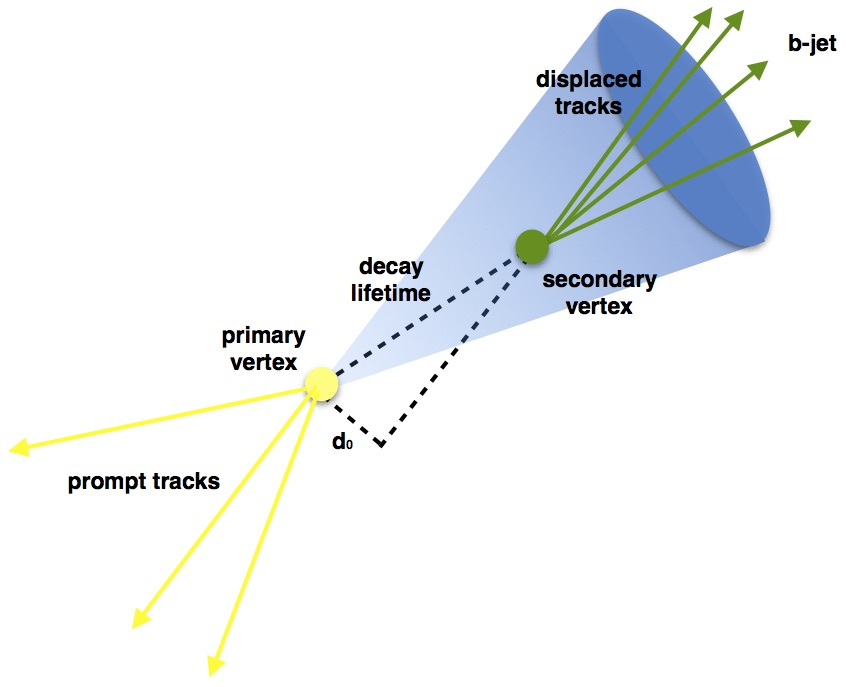
\includegraphics[width=\linewidth]{figures/chapter4/impact_parameters.png}
		\caption{}
		\label{fig:IP3D:d0}
	\end{subfigure}
  \hspace{0.1\textwidth}   % <-- space here
	\begin{subfigure}{.3\textwidth}
		\centering
		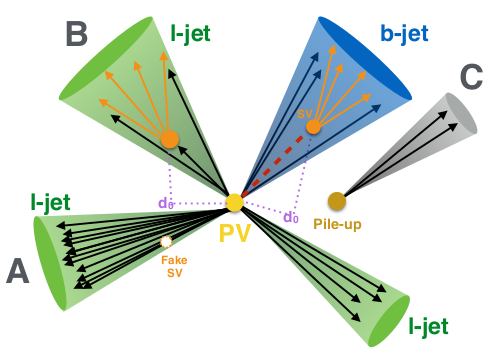
\includegraphics[width=\linewidth]{figures/chapter4/fake_SV.png}
		\caption{}
		\label{fig:IP3D:z0}
	\end{subfigure}
	\caption{https://www.hep.physik.uni-siegen.de/research/atlas/atlas-flavor-tagging}
	\label{fig:IP3D}
\end{figure}

The displacement of the secondary vertex can be characterized by the impact parameters of its associated tracks. The transverse impact parameter $d_0$ is the distance of closest approach between a track and the primary vertex in the transverse plane, while the longitudinal impact parameter $z_0$ is the corresponding distance along the beam axis. Tracks originating from a displaced B-hadron decay will exhibit statistically significant non-zero values of $d_0$ and $z_0$, providing a powerful discriminant against light-flavor jets whose tracks are consistent with the primary vertex. Charm hadrons also undergo displaced decays, though with a shorter mean lifetime ($\sim$0.5~ps) and correspondingly smaller average displacement, making c-jets a more challenging background to reject than light-flavor jets.

Early ATLAS b-tagging algorithms exploited these displaced-vertex signatures by combining track impact parameter significances, inclusive secondary vertex properties, and decay chain topology into multivariate discriminants, progressing from boosted decision trees to shallow and then deep neural networks. The following section describes the subsequent transition to end-to-end architectures that process the full set of tracks within a jet simultaneously, enabling substantial improvements in both light-jet and c-jet rejection.


\begin{figure}
	\centering
	\begin{subfigure}{.3\textwidth}
		\centering
		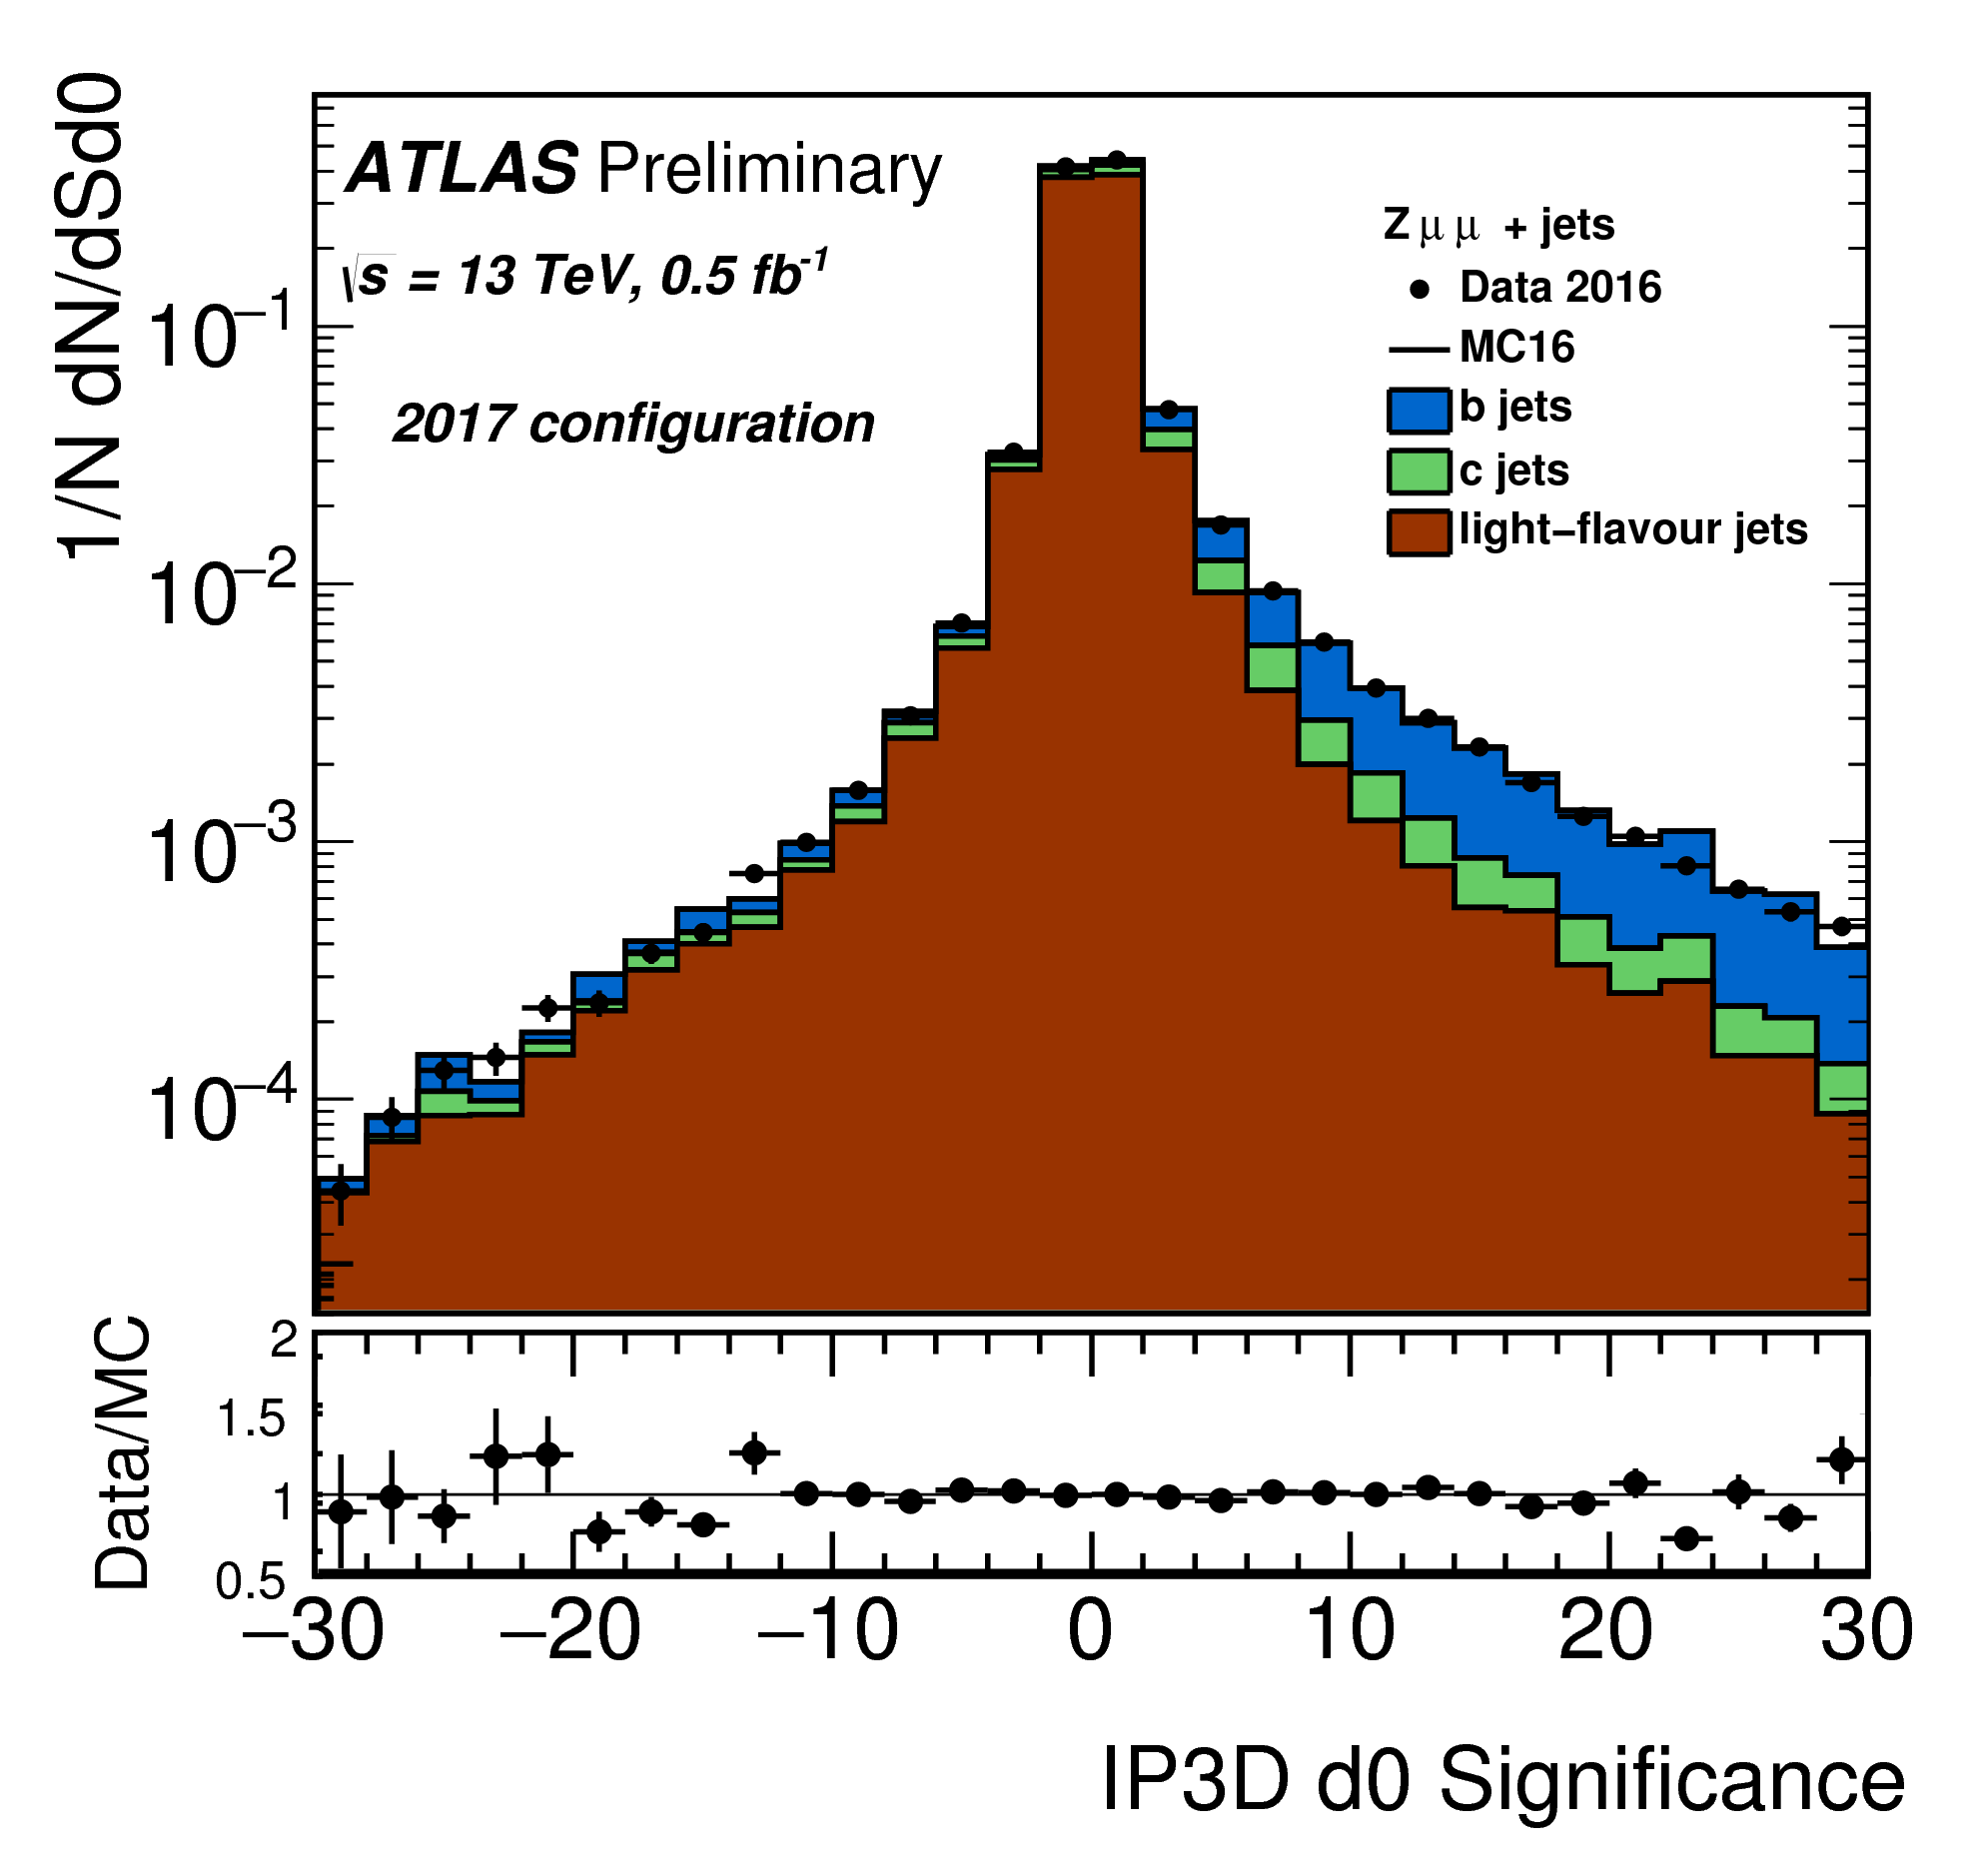
\includegraphics[width=\linewidth]{figures/chapter4/d0_sig.png}
		\caption{}
		\label{fig:IP3D:d0}
	\end{subfigure}
  \hspace{0.1\textwidth}   % <-- space here
	\begin{subfigure}{.3\textwidth}
		\centering
		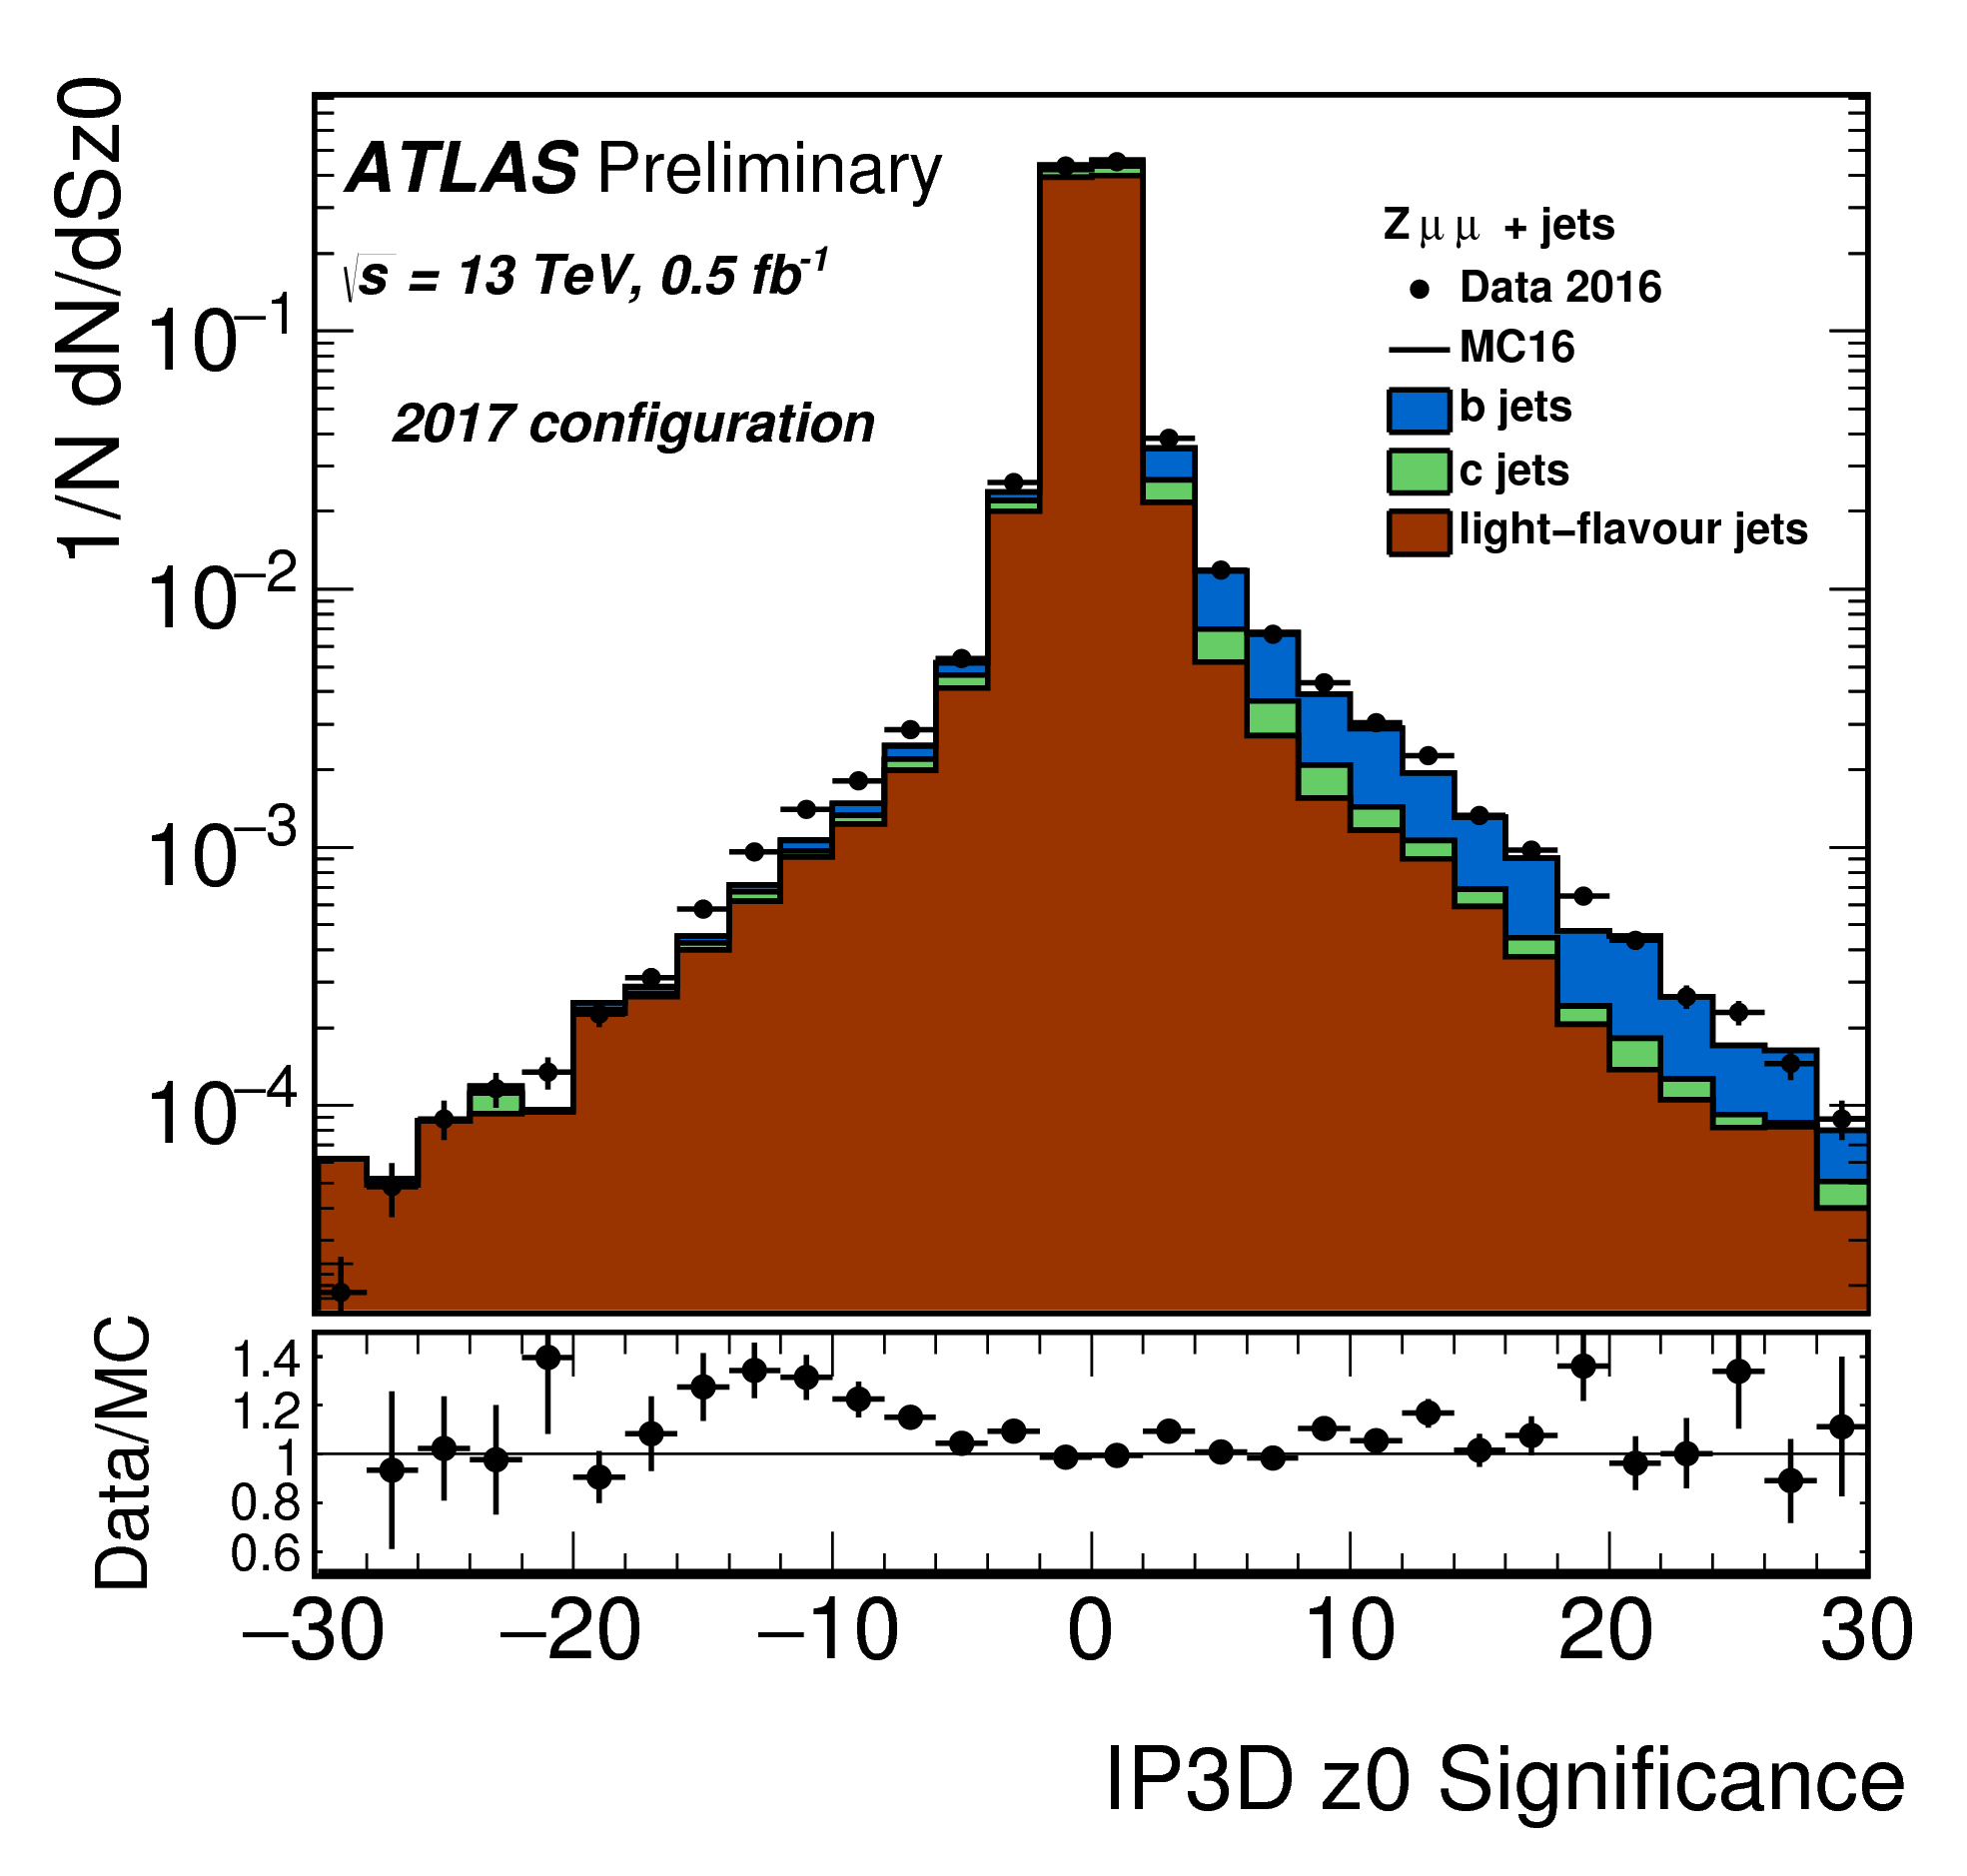
\includegraphics[width=\linewidth]{figures/chapter4/z0_sig.png}
		\caption{}
		\label{fig:IP3D:z0}
	\end{subfigure}
	\caption{https://atlas.web.cern.ch/Atlas/GROUPS/PHYSICS/PUBNOTES/ATL-PHYS-PUB-2017-013/}
	\label{fig:IP3D}
\end{figure}

\section{Overview of Architectures for Modeling Jets}

Jet flavor identification at the LHC is a multi-class classification problem: given a jet, a tagger must discriminate between b-jets, c-jets, and light-flavor jets. Deep neural networks (DNNs) are well suited to this task, learning non-linear decision boundaries in high-dimensional feature spaces directly from MC-simulated training samples where truth-level flavor labels are available. Crucially, architectures that operate directly on the full set of tracks within a jet, treating the jet as a variable-length set of objects, preserve information that is inevitably lost when constructing fixed-size high-level summary variables. The following subsections describe the graph and attention based architectures that exploit this, and the performance gains they deliver in both b-jet and c-jet identification.

\subsection{Graph Neural Networks and GN1}

\begin{figure}[h]
	\centering
	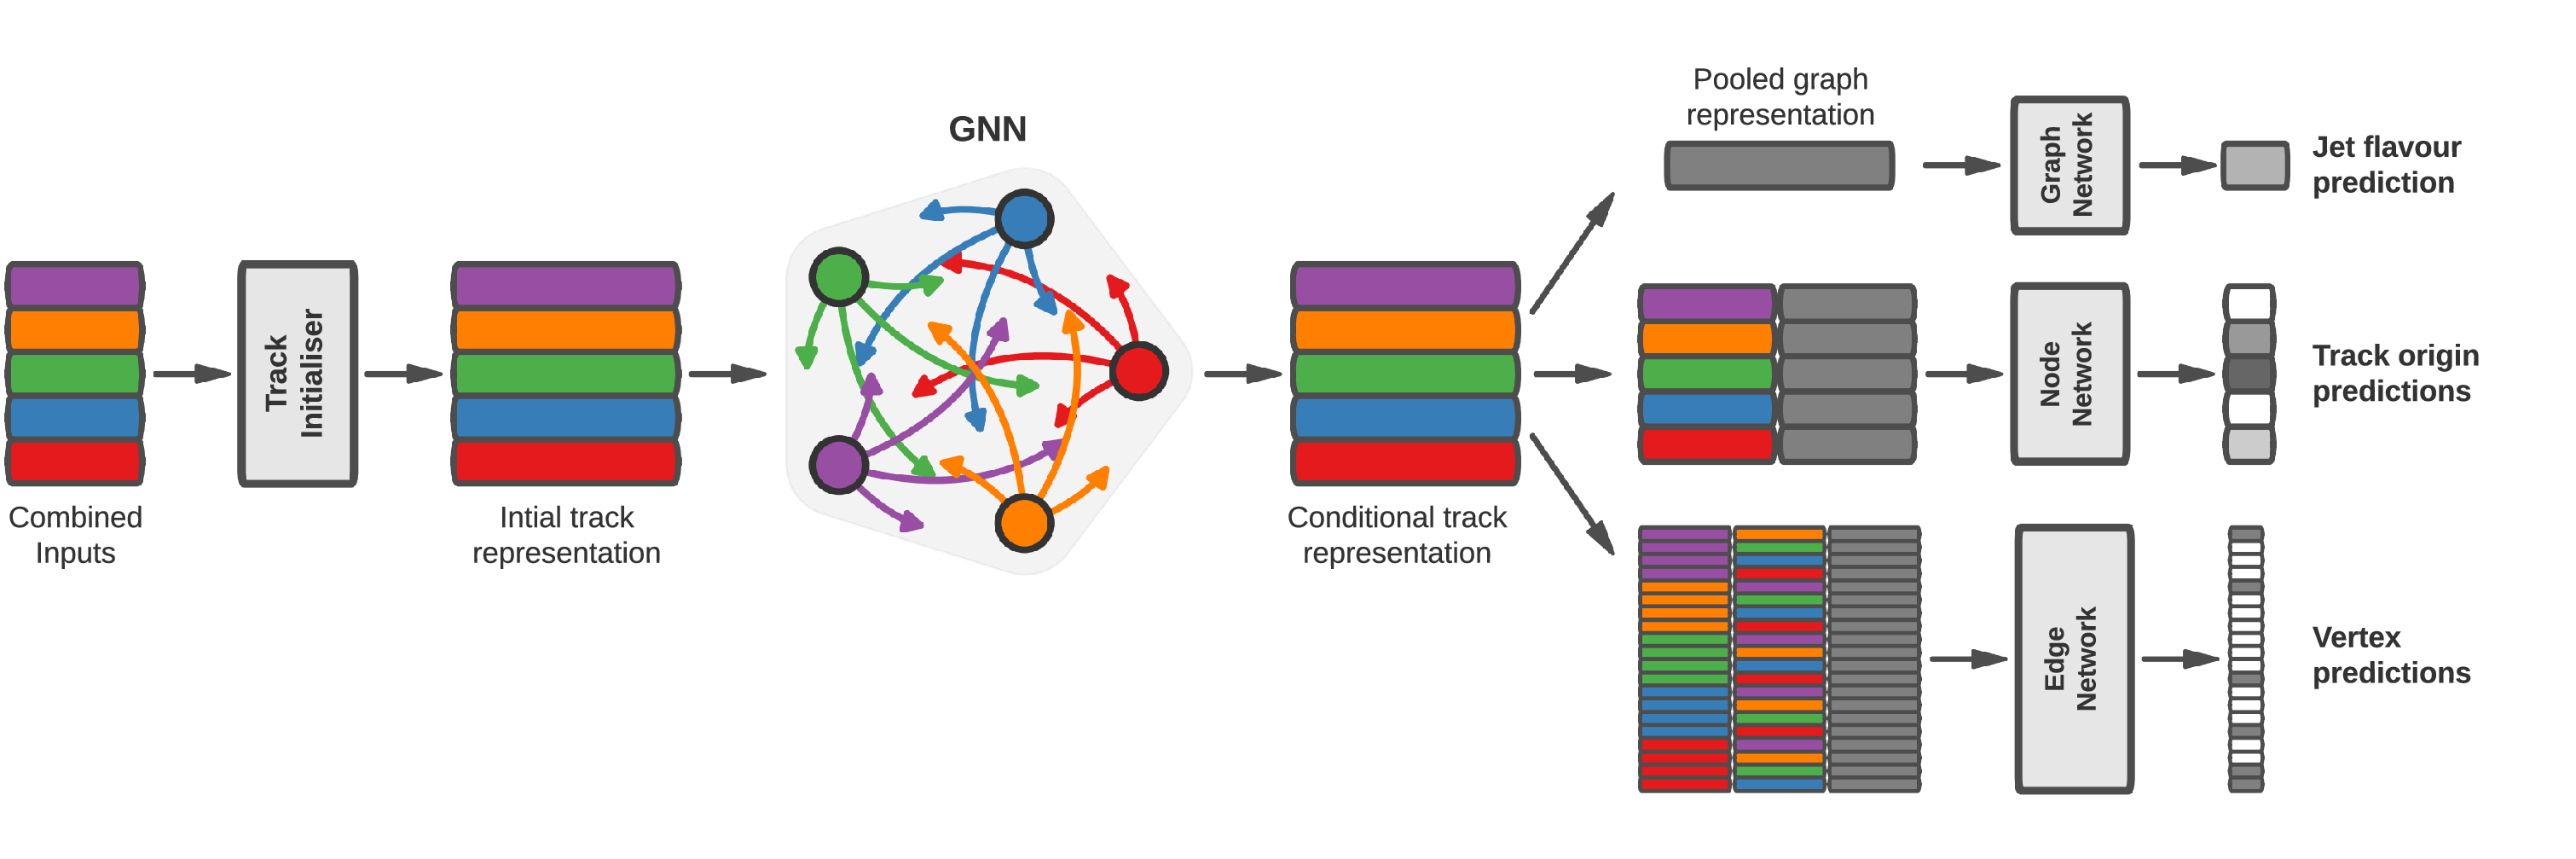
\includegraphics[width=1.0\linewidth]{figures/chapter4/GN1.png}
	\caption{https://atlas.web.cern.ch/Atlas/GROUPS/PHYSICS/PUBNOTES/ATL-PHYS-PUB-2022-027/}
	\label{fig:GN1}
\end{figure}

A graph neural network (GNN) represents a set of objects as nodes in a graph, with edges
encoding pairwise relationships between them. Message passing operations allow each node to
iteratively aggregate information from its neighbors, building representations that capture
both individual object properties and the collective structure of the ensemble. Formally, the
updated representation of node $i$ at layer $k$ is given by:
\begin{equation}
	\mathbf{x}_i^{(k)} = \gamma^{(k)} \!\left( \mathbf{x}_i^{(k-1)},\; \bigoplus_{j \in \mathcal{N}(i)} \phi^{(k)}\!\left( \mathbf{x}_i^{(k-1)}, \mathbf{x}_j^{(k-1)}, \mathbf{e}_{j,i} \right) \right)
\end{equation}
where $\mathbf{x}_i^{(k-1)} \in \mathbb{R}^F$ are the node features of node $i$, $\mathbf{e}_{j,i} \in \mathbb{R}^D$
are optional edge features, $\bigoplus$ denotes a differentiable permutation-invariant aggregation
function such as a sum, mean, or max, and $\gamma$ and $\phi$ are differentiable functions
implemented as MLPs. This is a natural fit for the tracks within a jet, which form an unordered
set with meaningful pairwise relationships such as angular separation or compatibility with a
common decay vertex.

https://pytorch-geometric.readthedocs.io/en/latest/notes/create\_gnn.html

\begin{figure}[h]
	\centering
	\begin{subfigure}[c]{.4\textwidth}
		\centering
		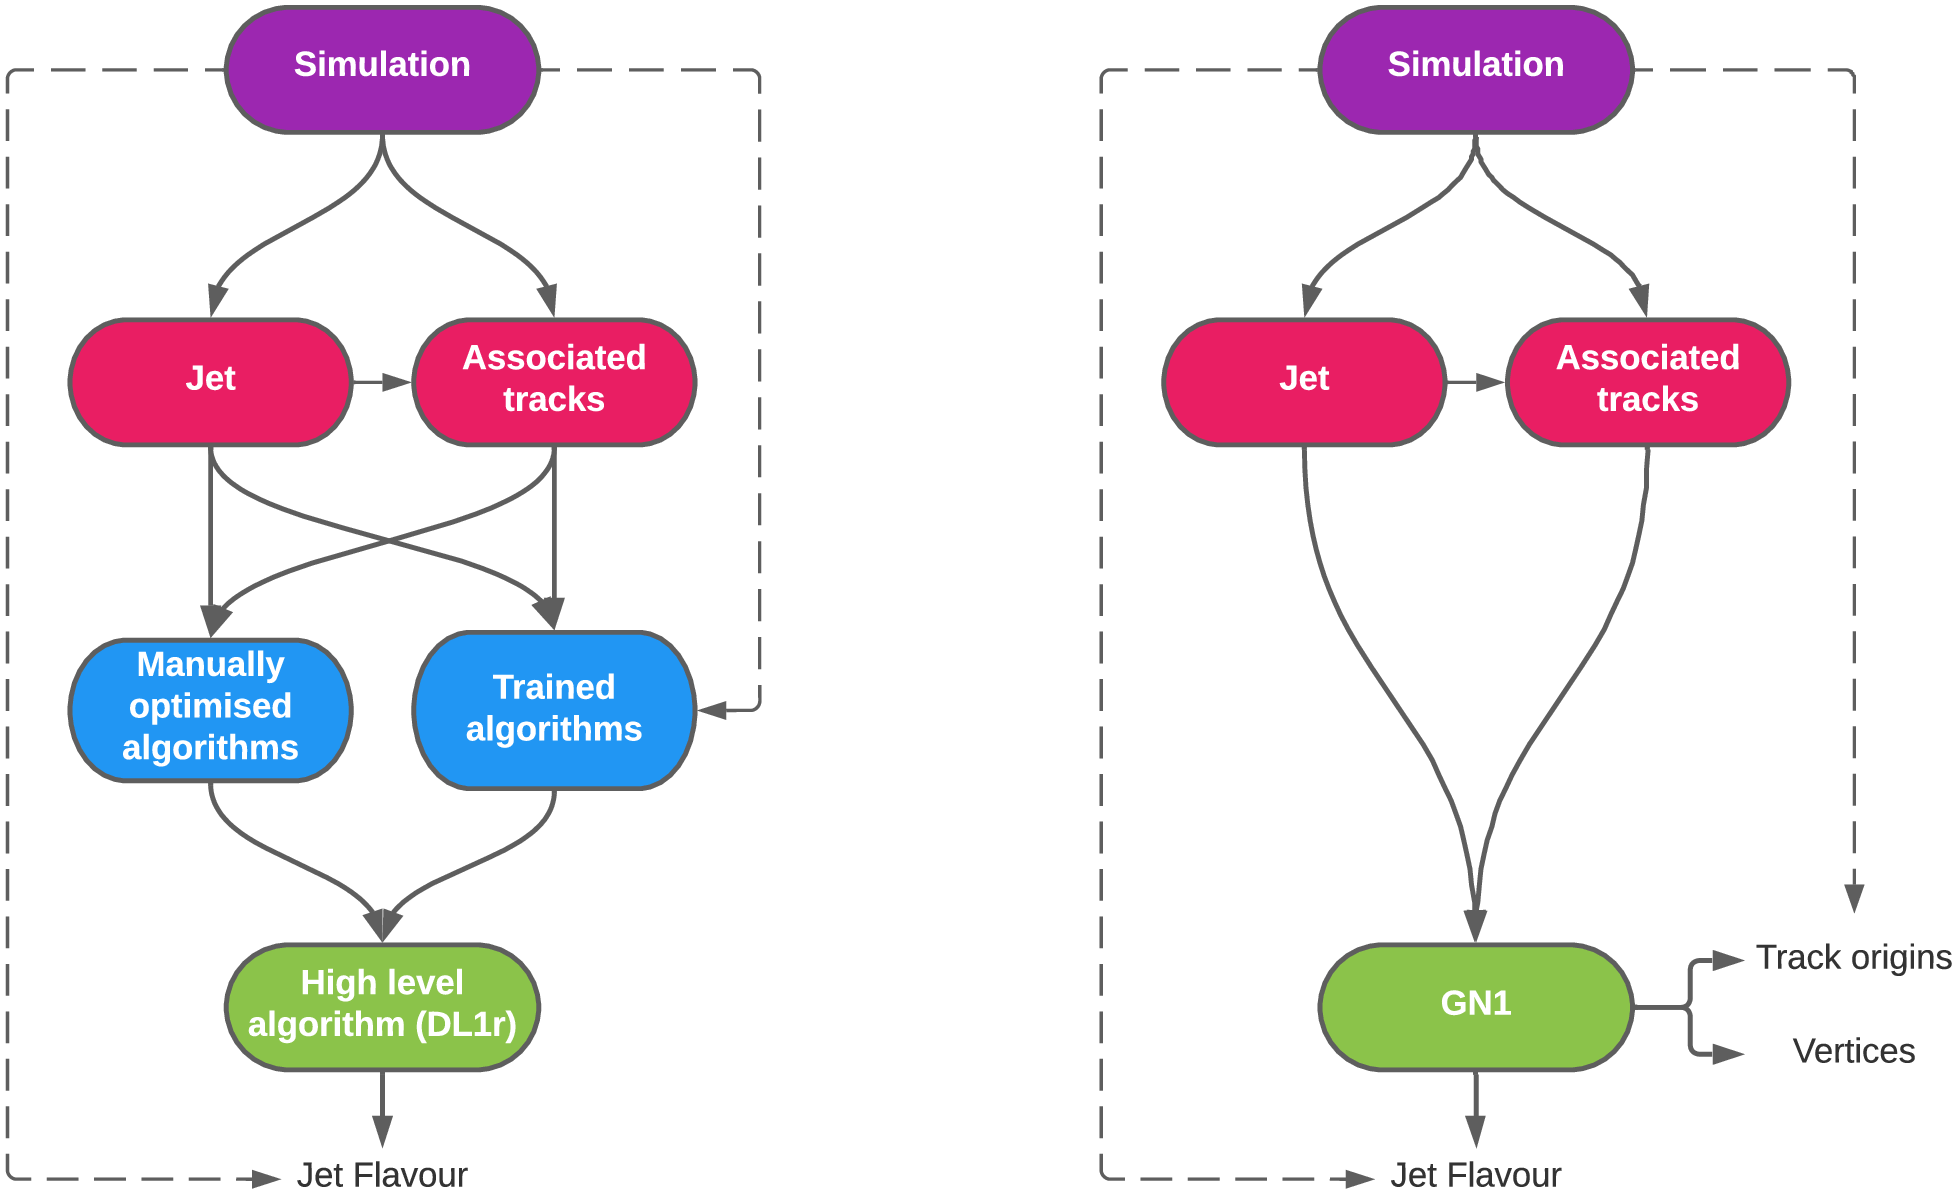
\includegraphics[width=\linewidth]{figures/chapter4/low_level_inputs.png}
		\caption{}
		\label{fig:IP3D:d0}
	\end{subfigure}
	\hspace{0.09\textwidth}   % <-- space here
	\begin{subfigure}[c]{.49\textwidth}
		\centering
		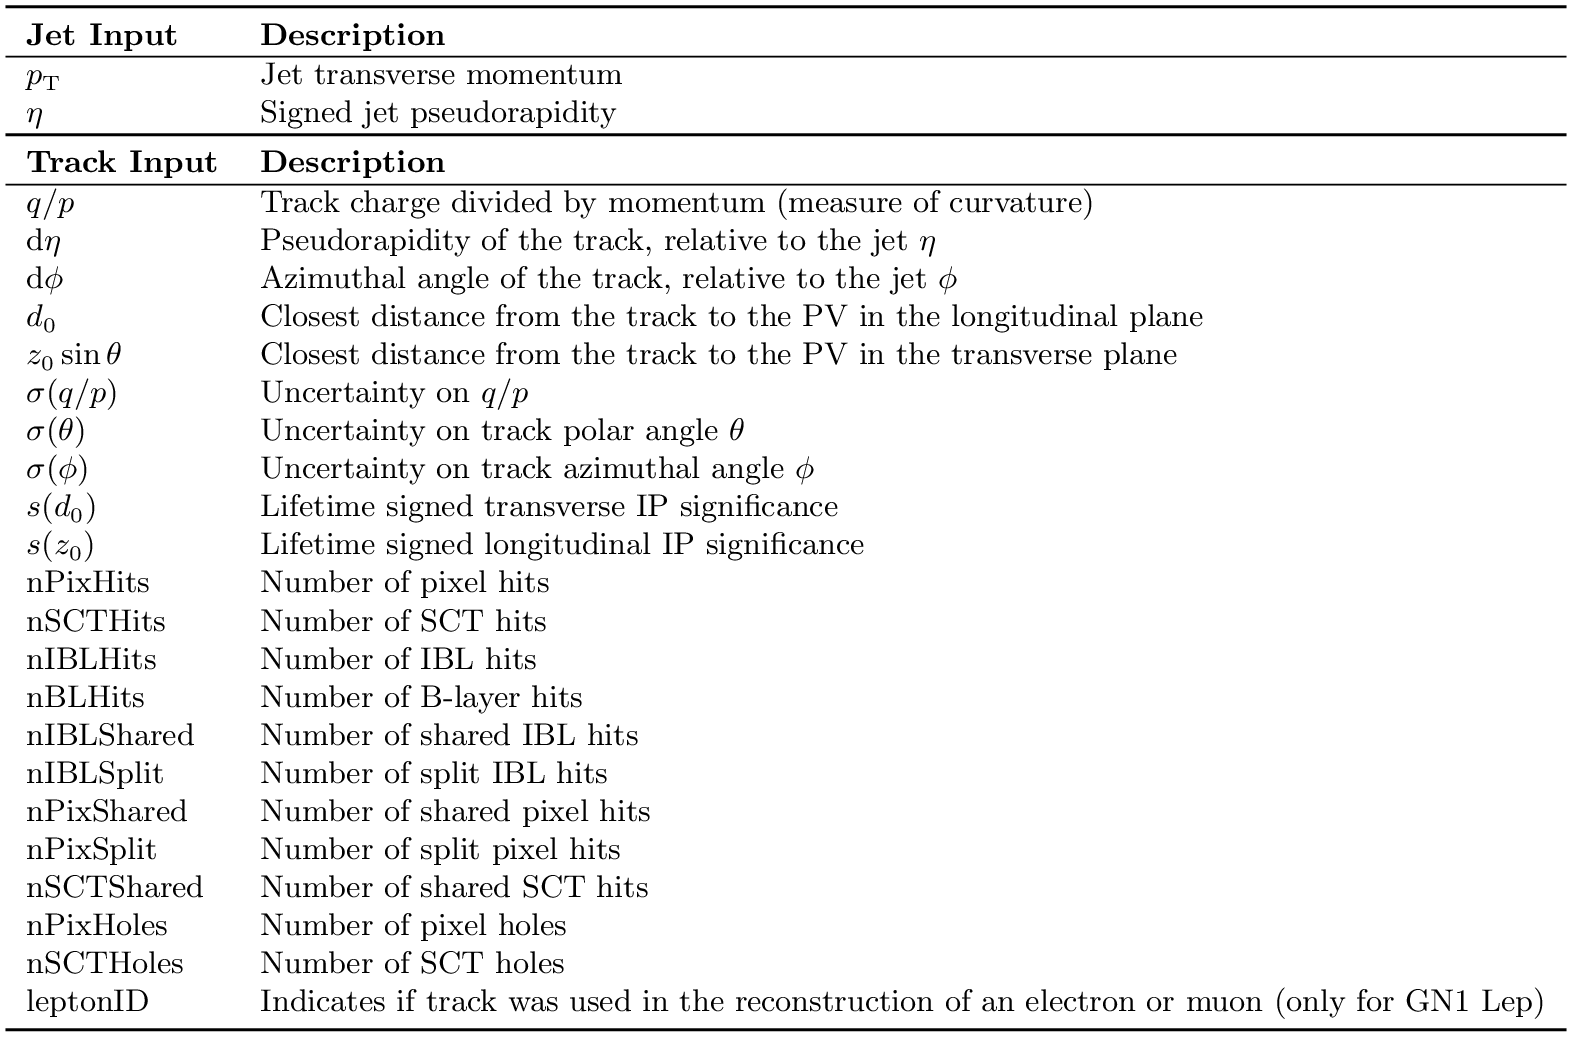
\includegraphics[width=\linewidth]{figures/chapter4/GN1_features.png}
		\caption{}
		\label{fig:IP3D:z0}
	\end{subfigure}
	\caption{https://atlas.web.cern.ch/Atlas/GROUPS/PHYSICS/PUBNOTES/ATL-PHYS-PUB-2022-027/}
	\label{fig:GN1_Inputs}
\end{figure}

\texttt{GN1} represented a fundamental architectural shift, moving away from the paradigm of
combining outputs of separately optimized low-level tagging algorithms towards a single
end-to-end graph-based representation of the jet. Tracks are treated as nodes in a fully
connected graph, with message passing used to build representations encoding both individual
track properties and the collective structure of the track ensemble. Rather than taking
pre-computed high-level discriminants as inputs, \texttt{GN1} operates directly on low-level
track parameters including impact parameter significances, track kinematics, and hit-level
variables such as pixel and SCT hit counts, exploiting information that is otherwise compressed
or discarded when constructing high-level summary variables.

\texttt{GN1} also introduced multi-task training with two auxiliary objectives alongside the
primary jet-level $b$/$c$/light classification. The first predicts the truth origin of each
individual track, classifying it as originating from the primary vertex, a $b$-hadron decay,
a $c$-hadron decay, pileup, or other secondary processes. The second predicts the vertex
compatibility of each pair of tracks, determining whether two tracks originate from the same
vertex and thereby performing implicit secondary vertex finding without a dedicated vertexing
algorithm. Together these auxiliary objectives act as powerful regularizers, encouraging the
network to build physically interpretable representations that generalize well across jet
kinematics. The graph-based message passing combined with multi-task learning produced
substantial improvements in both light-jet and $c$-jet rejection over \texttt{DL1r}.

\subsection{Attention Mechanism and Transformers and GN2}

\begin{figure}[h]
	\centering
	\begin{subfigure}[c]{.4\textwidth}
		\centering
		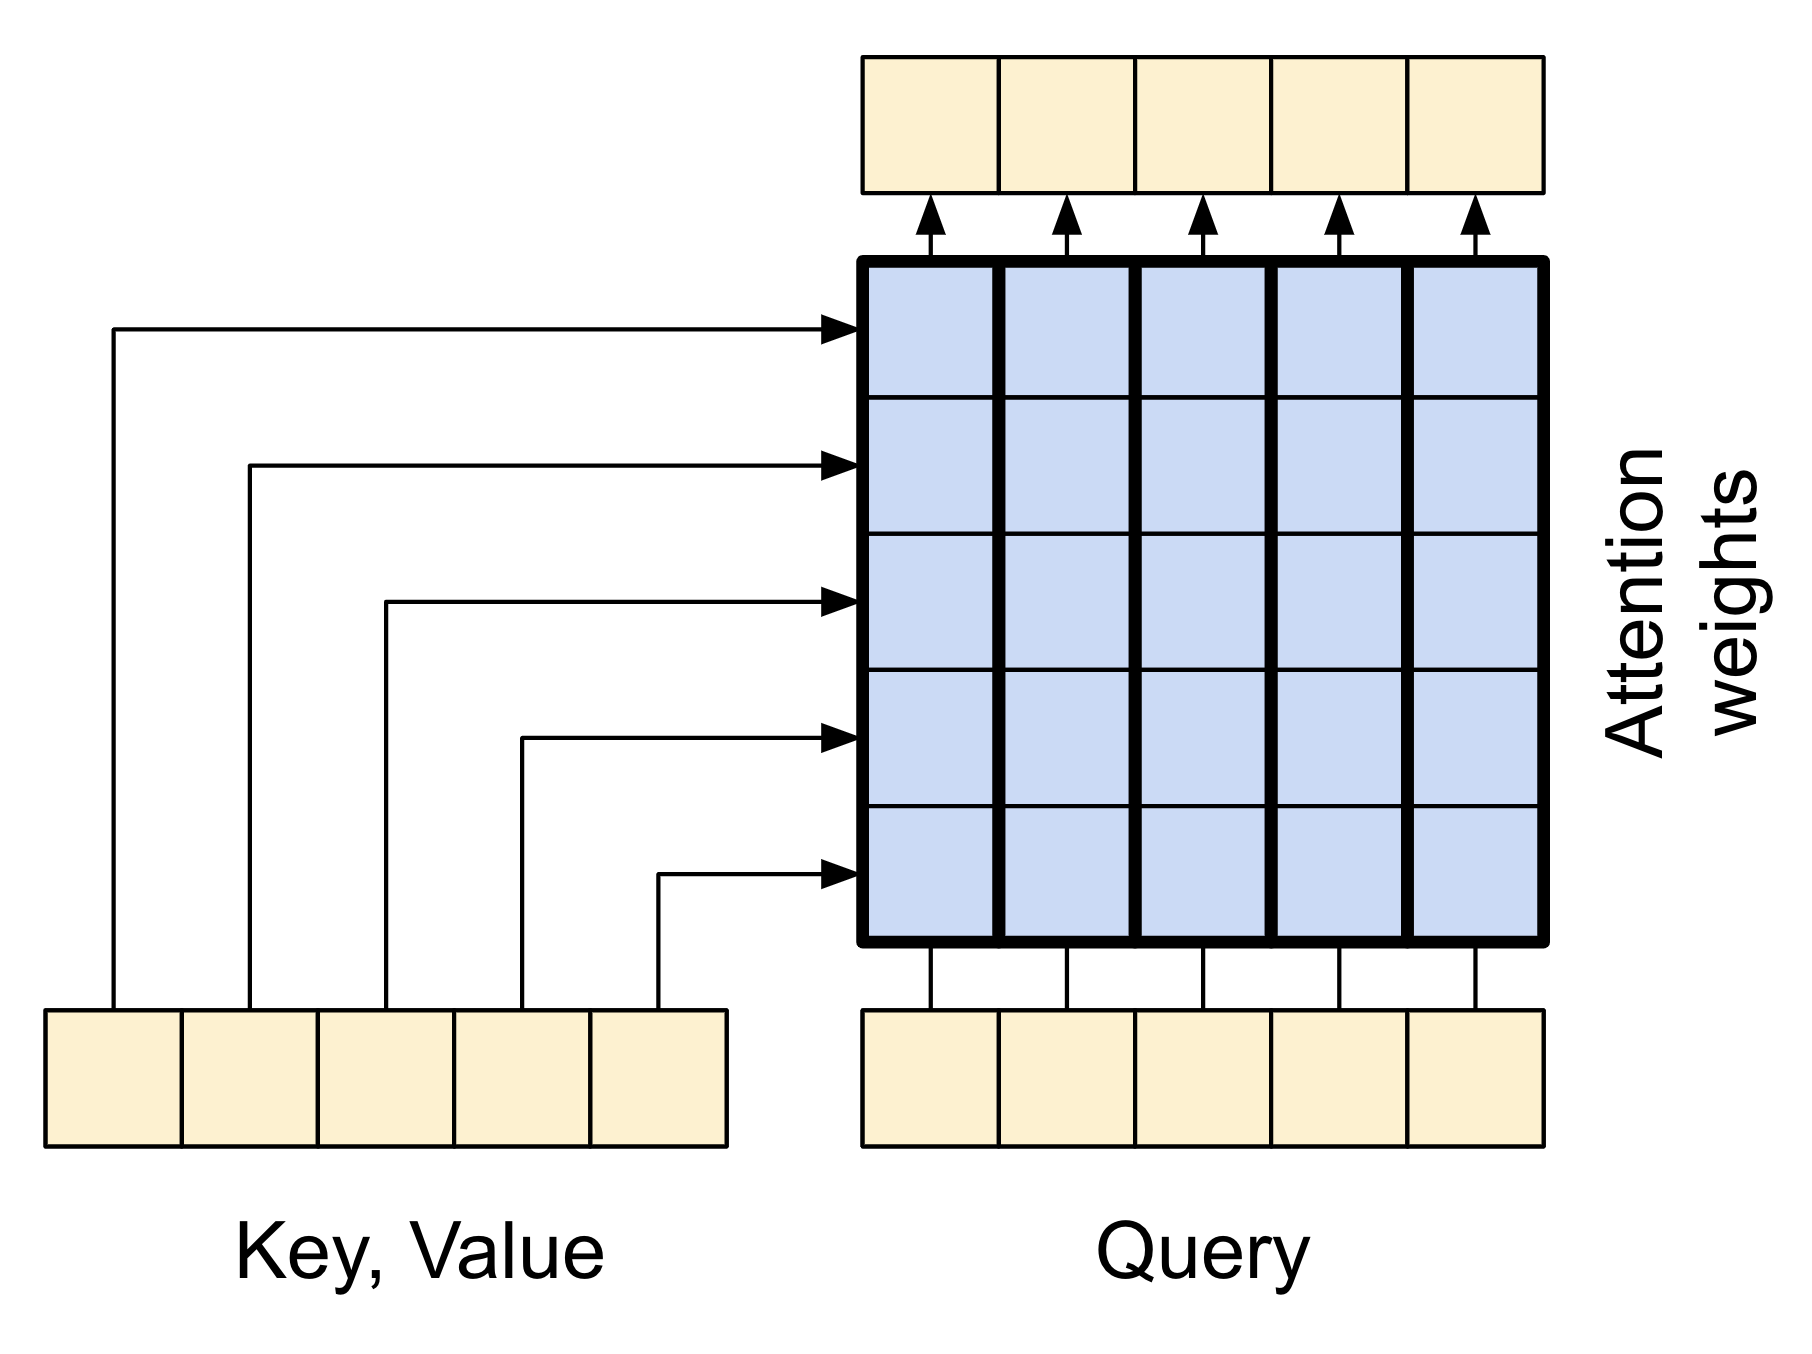
\includegraphics[width=\linewidth]{figures/chapter4/attention_weights.png}
		\caption{}
		\label{fig:attention_weights}
	\end{subfigure}
	\hspace{0.09\textwidth}   % <-- space here
	\begin{subfigure}[c]{.2\textwidth}
		\centering
		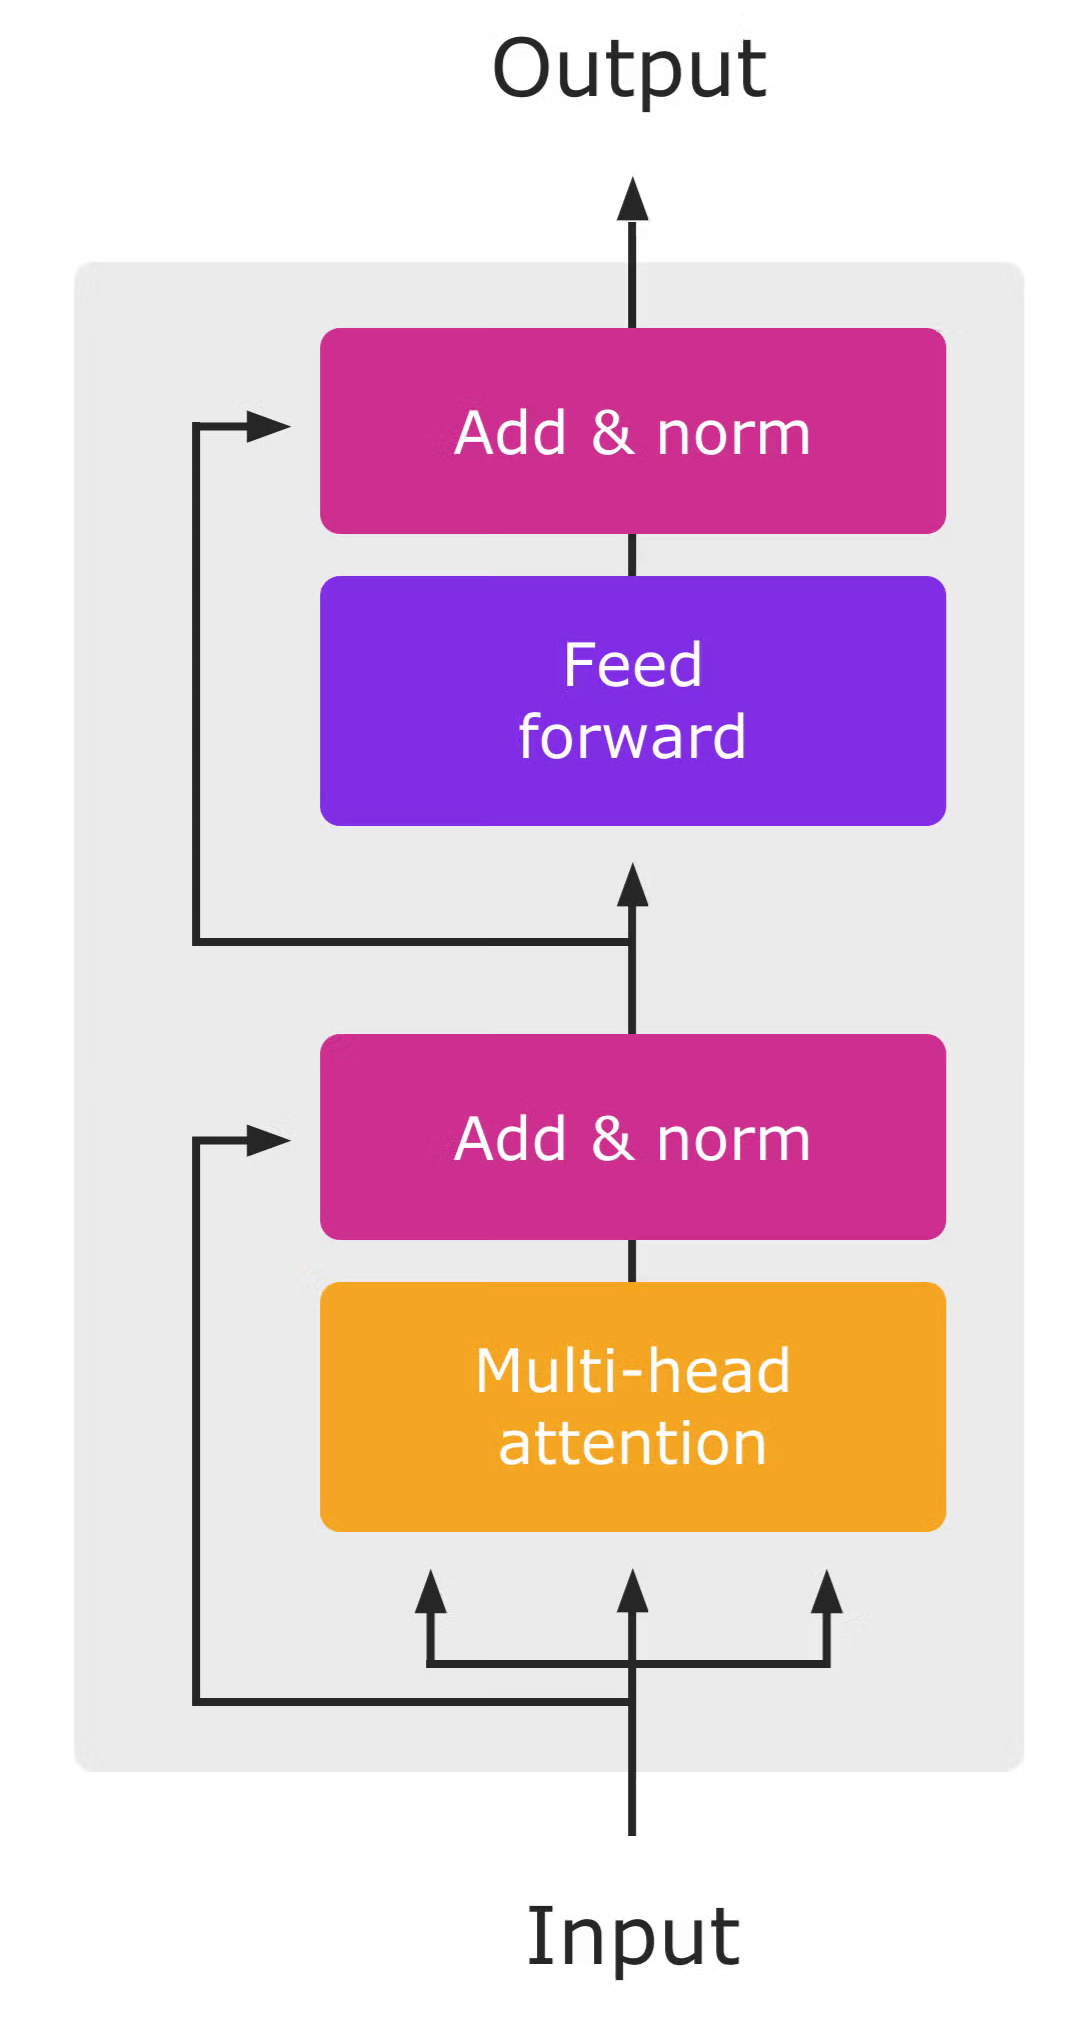
\includegraphics[width=\linewidth]{figures/chapter4/attention_encoder.png}
		\caption{}
		\label{fig:attention_encoder}
	\end{subfigure}
	\caption{https://atlas.web.cern.ch/Atlas/GROUPS/PHYSICS/PUBNOTES/ATL-PHYS-PUB-2022-027/}
	\label{fig:attention}
\end{figure}

The attention mechanism computes updated representations of each element in a set by learning
dynamic edge weights that reflect the correlations, or local context, between all pairs of
elements. In scaled dot-product attention, each object's representation is projected into three
vectors: a query $\mathbf{q}$, a key $\mathbf{k}$, and a value $\mathbf{v}$. Collecting these
projections across all $N$ objects into matrices $Q$, $K$, and $V$, the updated representations
are given by:
\begin{equation}
	\text{Attention}(Q, K, V) = \text{softmax}\!\left(\frac{QK^\top}{\sqrt{d_k}}\right)V
\end{equation}
where $d_k$ is the dimension of the key vectors, introduced to prevent saturation of the softmax
at large dot-product magnitudes. For a jet with $N$ tracks, this produces an $N \times N$
attention matrix at each layer, where entry $(i,j)$ reflects how strongly track $i$ attends to
track $j$ when updating its representation. A transformer encoder block consists of one such
self-attention operation followed by a position-wise feed-forward network, with residual
connections and layer normalization around both. Multi-head attention extends this by running
$h$ independent attention operations in parallel with separate learned projections, allowing the
network to simultaneously capture different aspects of the track relationships.

Compared to the message passing approach of \texttt{GN1}, self-attention offers several
advantages for jet flavor tagging. In message passing, all neighboring tracks contribute to
the node update through a fixed aggregation function, regardless of their relevance to the jet.
Self-attention replaces this with a fully learned, input-dependent weighting, allowing the
network to dynamically identify which track pairs are most discriminating on a per-jet basis.
This enables the capture of long-range correlations across the full track ensemble without any
locality bias. The learned attention weights also provide direct interpretability: they can be
inspected to understand which track pairs the network considers most informative for a given
tagging decision, as illustrated in Figure~\ref{fig:attention}.

\texttt{GN2} extended \texttt{GN1} by replacing the message passing aggregation with a
transformer encoder applied directly to the set of tracks within each jet. The multi-task
training objectives of \texttt{GN1} were retained, and the input feature set was extended to
include additional track quality and vertex variables. A global jet representation is formed by
an attention-weighted sum over the final track representations and passed to the jet-level
classification head. \texttt{GN2} currently represents the state-of-the-art resolved jet
flavor tagger deployed in ATLAS, achieving the best light-jet and $c$-jet rejection of any
tagger in the sequence, and forming the architectural basis for the boosted jet tagger
\texttt{GN2X} described in Section~\ref{sec:boosted}.

\subsection{Benchmarks and Results -- Resolved}

The performance of a flavor tagger is evaluated using a receiver operating characteristic (ROC)
curve. The tagger produces a continuous discriminant score for each jet, and a working point is
defined by placing a threshold on this score. By scanning the threshold continuously, one traces
out a curve in the space of signal efficiency and background rejection, where the signal
efficiency is the fraction of true $b$-jets passing the threshold and the background rejection
is the inverse of the false positive rate. In HEP it is conventional to plot the light-jet
rejection $1/\varepsilon_\text{light}$ and $c$-jet rejection $1/\varepsilon_c$ as functions of
the $b$-jet efficiency $\varepsilon_b$. The area under the curve (AUC) provides a single
threshold-independent summary of overall tagger performance. Specific working points ---
typically $\varepsilon_b = 60\%$, $70\%$, $77\%$, and $85\%$ --- are defined by fixing the
$b$-jet efficiency and quoting the corresponding background rejection, allowing direct comparison
between taggers and across analyses.

Figure~\ref{fig:GN1:results} shows the output discriminant distributions and ROC curves for
\texttt{DL1r} and \texttt{GN1}, evaluated on a simulated $t\bar{t}$ sample with
$20 < p_\text{T} < 250$~GeV at $\sqrt{s} = 13$~TeV. The $b$-jet distributions are peaked at
high discriminant values while the $c$-jet and light-jet distributions are concentrated at lower
values; the \texttt{GN1} distributions show a more pronounced separation between all three
flavors relative to \texttt{DL1r}. The dashed vertical lines indicate the $60\%$ and $80\%$
$b$-jet efficiency working points. The ROC curves confirm this improvement quantitatively: at
the $70\%$ working point, \texttt{GN1} achieves approximately 1.8 times greater light-jet
rejection and 2.1 times greater $c$-jet rejection than \texttt{DL1r}, with the ratio panels
showing a consistent gain across the full efficiency range.

\begin{figure}[h]
	\centering
	\begin{subfigure}[c]{.4\textwidth}
		\centering
		\includegraphics[width=\linewidth]{figures/chapter4/GN1_discriminant.png}
		\caption{}
		\label{fig:GN1:discriminant}
	\end{subfigure}
	\hspace{0.05\textwidth}   % <-- space here
	\begin{subfigure}[c]{.43\textwidth}
		\centering
		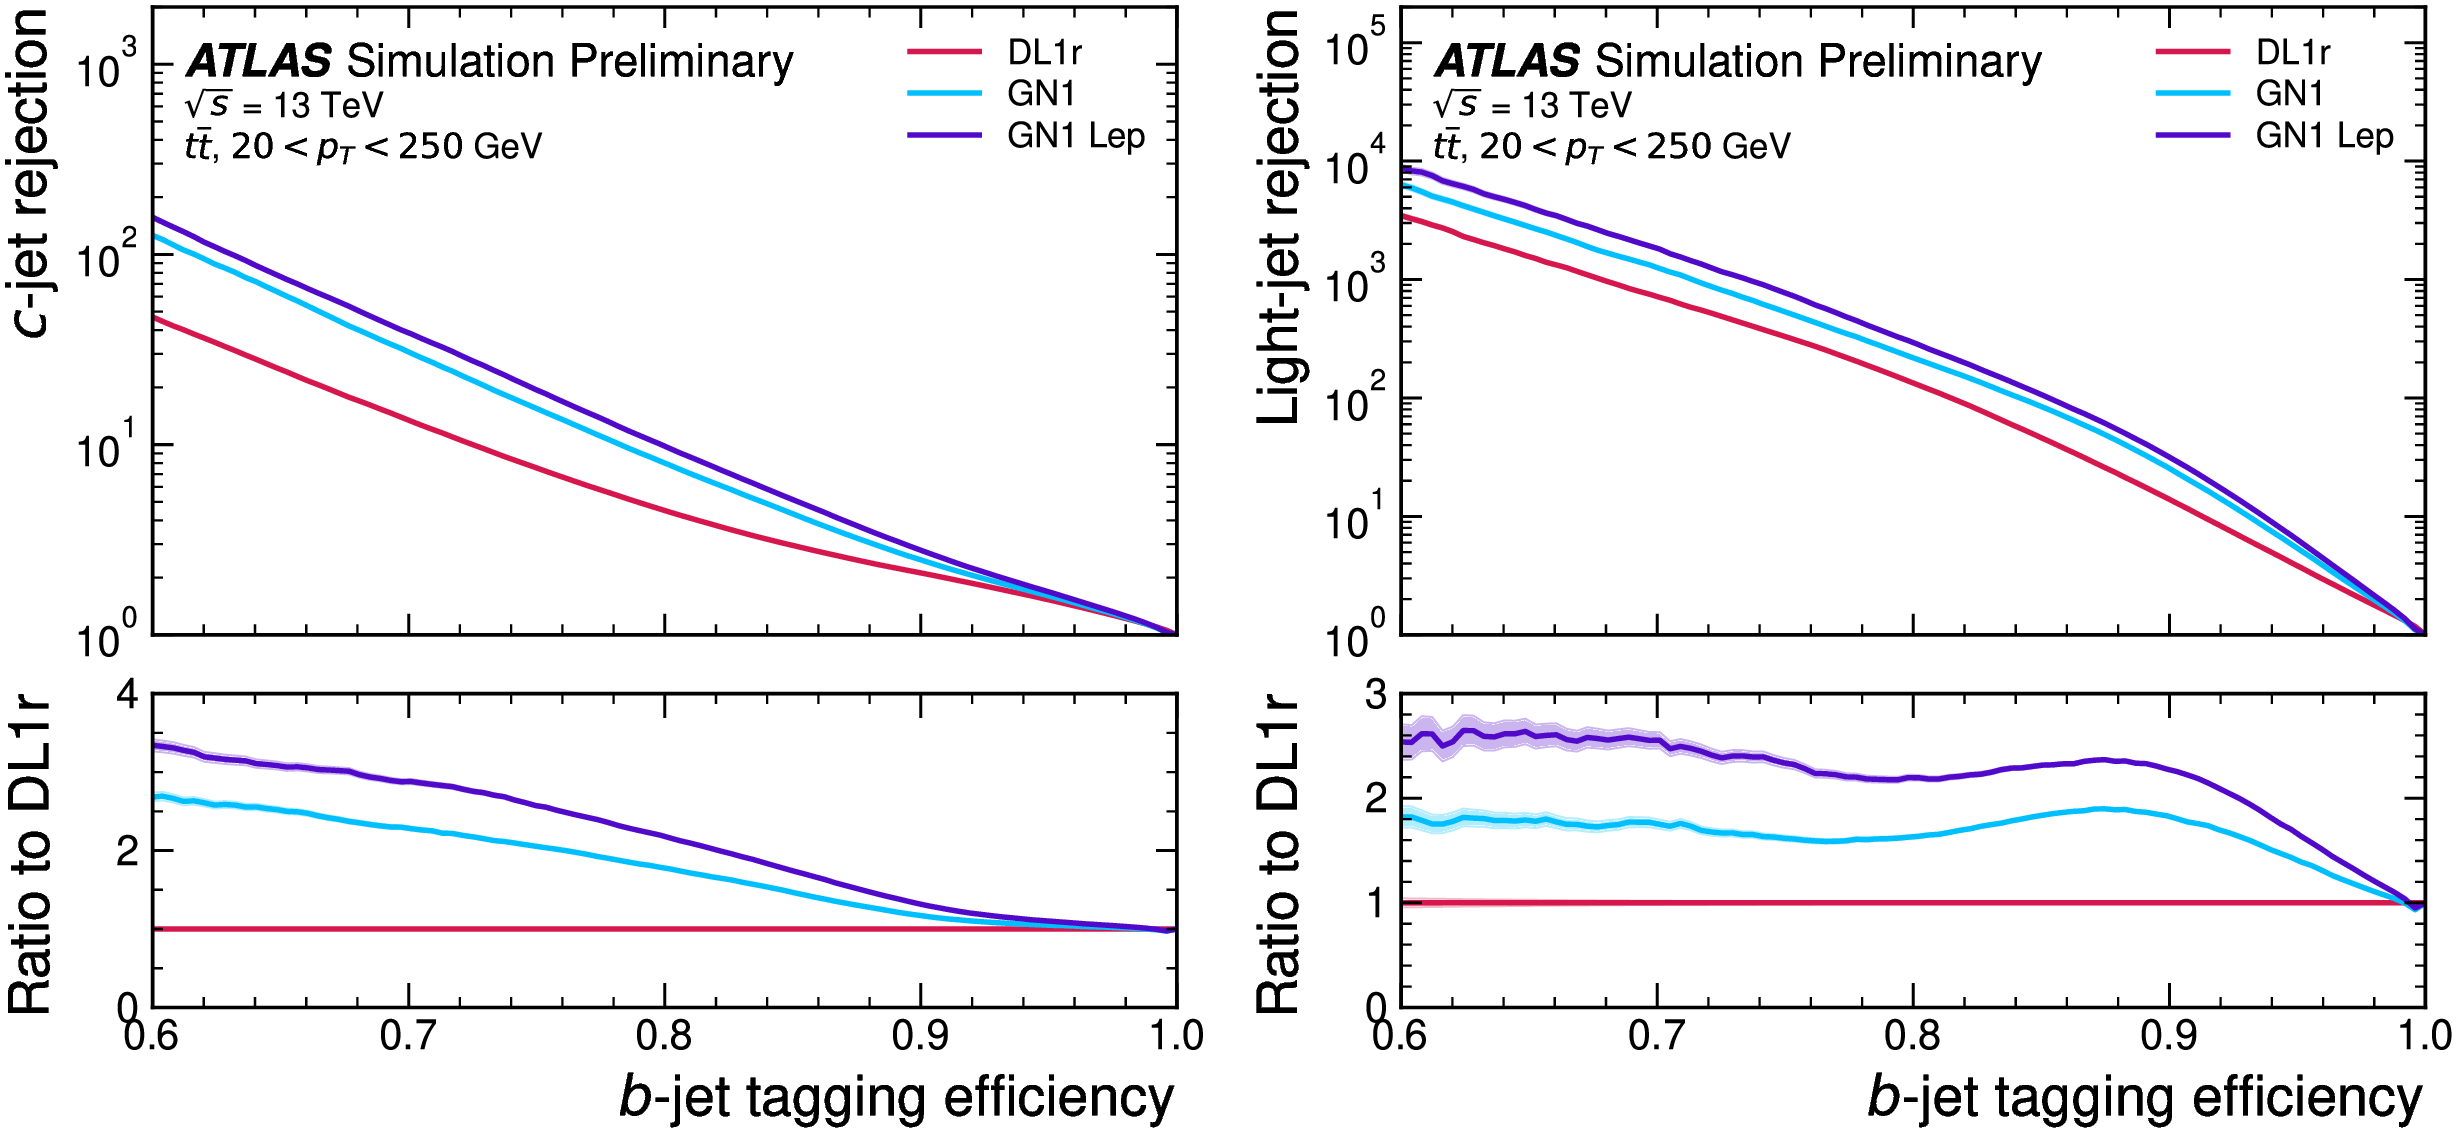
\includegraphics[width=\linewidth]{figures/chapter4/GN1_b_ROC.png}
		\caption{}
		\label{fig:GN1:ROC}
	\end{subfigure}
	\caption{https://atlas.web.cern.ch/Atlas/GROUPS/PHYSICS/PUBNOTES/ATL-PHYS-PUB-2022-027/}
	\label{fig:GN1:results}
\end{figure}

Figure~\ref{fig:GN2:results} shows the ROC curves for \texttt{DL1d}, \texttt{GN1}, and
\texttt{GN2}, comparing light-jet and $c$-jet rejection as a function of $b$-jet efficiency on
the same $t\bar{t}$ sample. Each successive architecture provides a clear improvement in
background rejection at fixed $b$-jet efficiency across the full range of working points. The
$c$-jet rejection improvements are more modest than those for light-jets, reflecting the
inherently smaller separation between $b$-jets and $c$-jets due to their shared heavy-flavor
decay topology. The cumulative performance gains across all three generations of taggers are
summarized in Figure~\ref{fig:history}.

\begin{figure}[h]
	\centering
	\begin{subfigure}[c]{.35\textwidth}
		\centering
		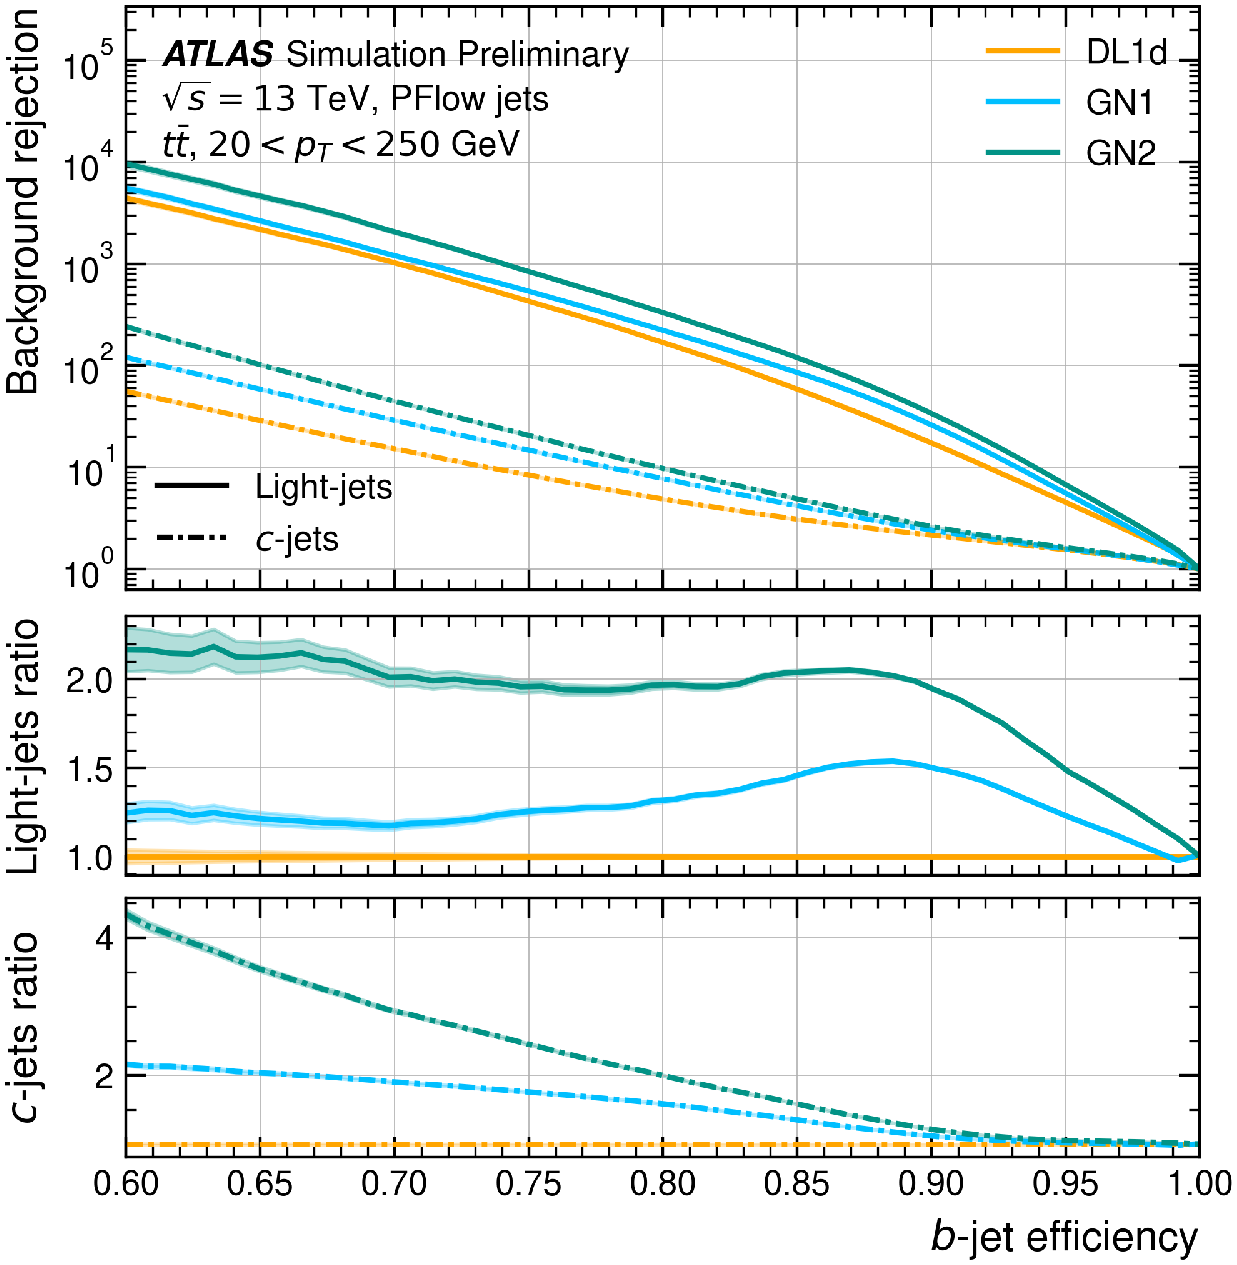
\includegraphics[width=\linewidth]{figures/chapter4/GN2_b_ROC.png}
		\caption{}
		\label{fig:GN2:b_ROC}
	\end{subfigure}
	\hspace{0.1\textwidth}   % <-- space here
	\begin{subfigure}[c]{.35\textwidth}
		\centering
		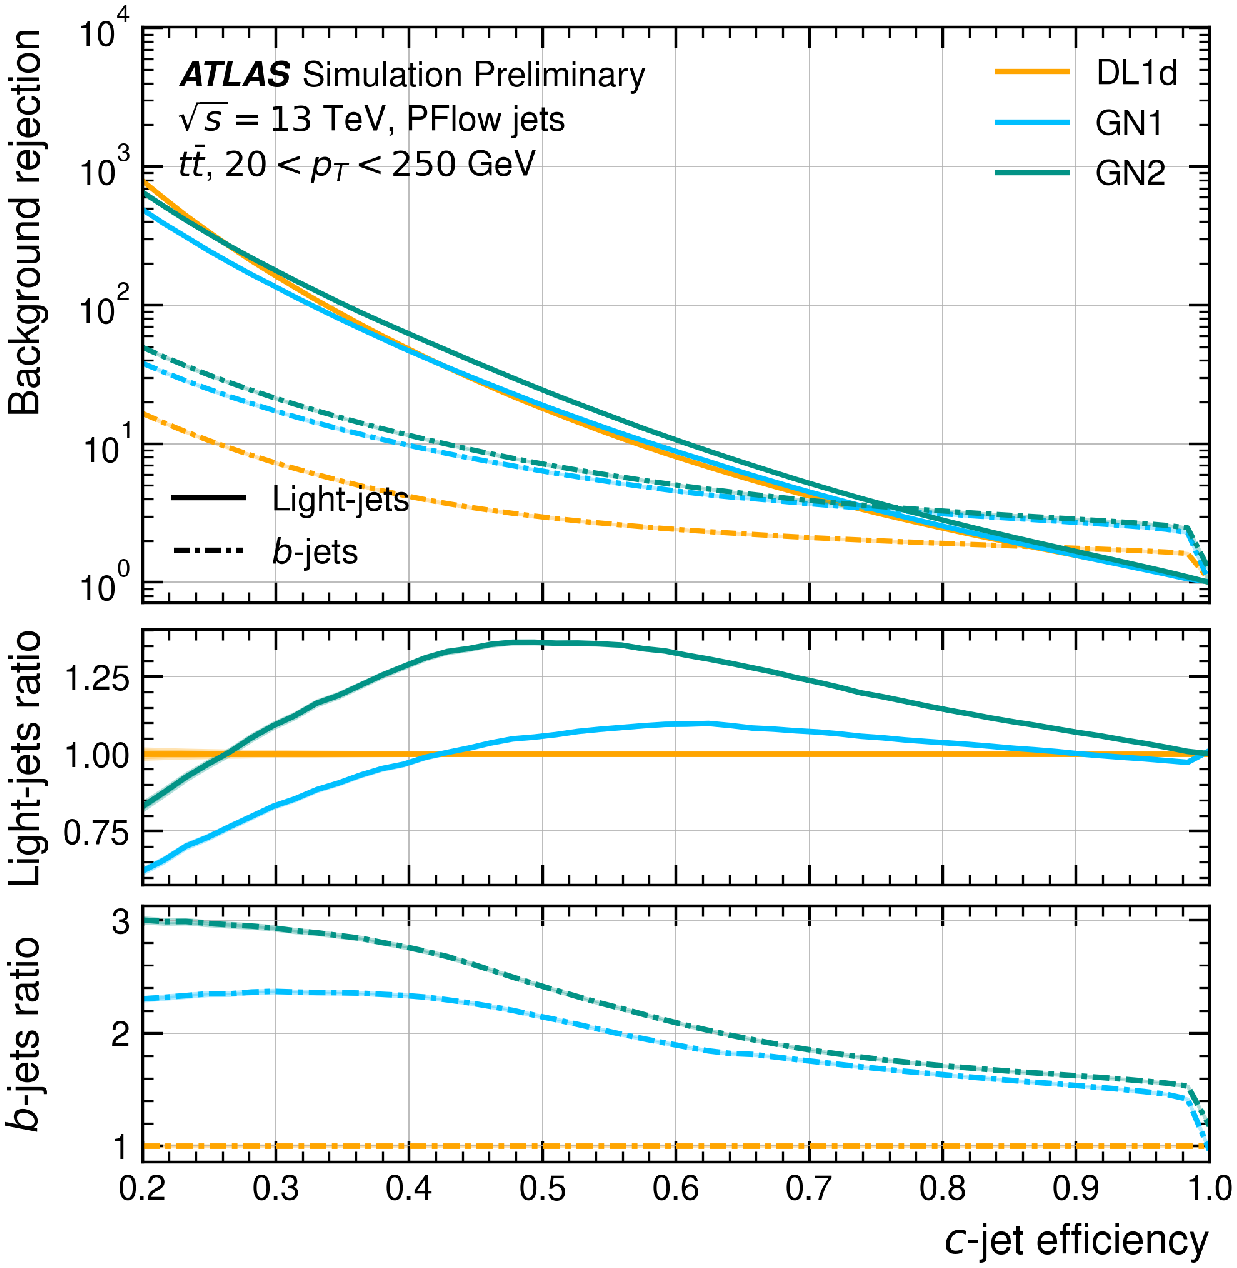
\includegraphics[width=\linewidth]{figures/chapter4/GN2_c_ROC.png}
		\caption{}
		\label{fig:GN2:c_ROC}
	\end{subfigure}
	\caption{https://atlas.web.cern.ch/Atlas/GROUPS/PHYSICS/PLOTS/FTAG-2023-01/}
	\label{fig:GN2:results}
\end{figure}

\begin{figure}[h]
	\centering
	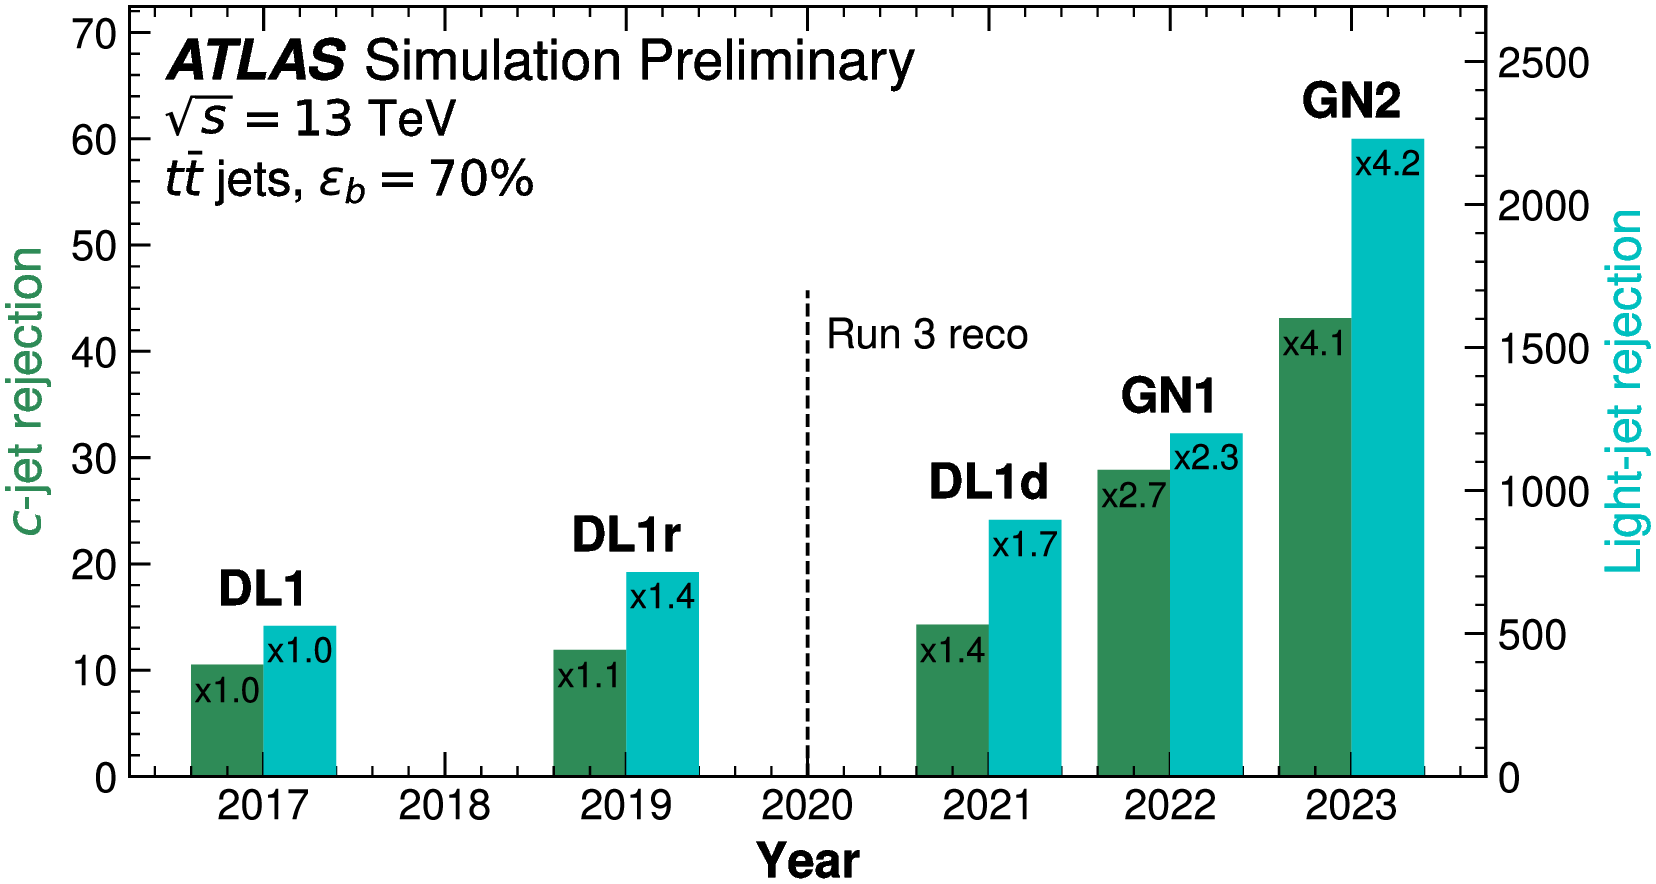
\includegraphics[width=0.7\linewidth]{figures/chapter4/performance_bar_graph.png}
	\caption{https://atlas.web.cern.ch/Atlas/GROUPS/PHYSICS/PLOTS/FTAG-2023-01/}
	\label{fig:history}
\end{figure}

\subsection{Boosted Jet Tagging with Graph and Attention Neural Networks}
\label{sec:boosted}

In addition to small-$R$ jet tagging, large-$R$ jet tagging ($R=1.0$) is used to identify boosted
objects whose decay products are sufficiently collimated that they cannot be resolved as individual
small-$R$ jets. Identifying these boosted jets is crucial for the Higgs program at the LHC, where
a boosted Higgs boson can hadronically decay via $H \rightarrow b\bar{b}$ and
$H \rightarrow c\bar{c}$, with multijet (QCD) processes and fully hadronic top-quark decays
forming the primary backgrounds. The previous state-of-the-art tagger, DXbb, combined
flavor-tagging discriminants from individual variable-radius (VR) subjets in a feed-forward
neural network, limiting its ability to exploit correlations between the decay products of both
$b$- and $c$-hadrons within the jet.

Building upon the transformer architecture of \texttt{GN2}, \texttt{GN2X} extends this approach
to large-$R$ jet tagging by operating directly on charged particle tracks associated with the
large-$R$ jet, reconstructed from Unified Flow Objects (UFOs). Up to 100 tracks are used as
input, sorted by decreasing transverse impact parameter significance, with each track described
by 20 variables including impact parameter significances, track kinematics, and hit-level
quantities. The network retains the multi-task training objectives of \texttt{GN1} and
\texttt{GN2}, simultaneously training track origin classification and vertex grouping auxiliary
tasks alongside the primary jet-level classification. Track representations are processed through
a transformer encoder consisting of 6 encoder blocks with 4 attention heads, and a global jet
representation is formed via an attention-weighted sum over the final track representations.
\texttt{GN2X} produces four probability scores via a softmax output layer: $p_{Hbb}$, $p_{Hcc}$,
$p_{\text{top}}$, and $p_{\text{QCD}}$.

These four probabilities are combined into a discriminant score taking the form of a log-likelihood
ratio:

\begin{align}
	D^{\text{GN2X}}_{Hbb} &= \ln \left( \frac{p_{Hbb}}{f_{Hcc} \cdot p_{Hcc} + f_{top} \cdot 
		p_{top} + (1 - f_{Hcc} - f_{top}) \cdot p_{QCD}} \right) \\
	D^{\text{GN2X}}_{Hcc} &= \ln \left( \frac{p_{Hcc}}{f_{Hbb} \cdot p_{Hbb} + f_{top} \cdot 
		p_{top} + (1 - f_{Hbb} - f_{top}) \cdot p_{QCD}} \right)
\end{align}

where $f_{Hcc}$ and $f_{\text{top}}$ are free parameters controlling the relative rejection weights
of the $H(c\bar{c})$ and top backgrounds with respect to multijet, optimized to maximize background
rejection at a given signal efficiency. For $H(b\bar{b})$ tagging, values of $f_{Hcc} = 0.02$ and
$f_{\text{top}} = 0.25$ are used~\cite{ATL-PHYS-PUB-2023-021}.

Working points are defined by placing a threshold on the discriminant score at a fixed signal
efficiency $\varepsilon_\text{sig}$, with looser working points retaining more signal at the cost
of greater background contamination, and tighter working points suppressing more background at the
cost of signal statistics. Figure~\ref{fig:GN2X_Discriminant} shows the normalized
$D^{\text{GN2X}}_{Hbb}$ discriminant distributions for all four jet classes evaluated on SM
samples with $p_\text{T} > 250$~GeV and $50 < m_J < 200$~GeV, with the dashed line indicating
the 50\% $H(b\bar{b})$ signal efficiency working point. The clear separation between the
$H(b\bar{b})$ distribution and the three background classes demonstrates the discriminating power
of the tagger.

\begin{figure}[htbp]
	\centering
	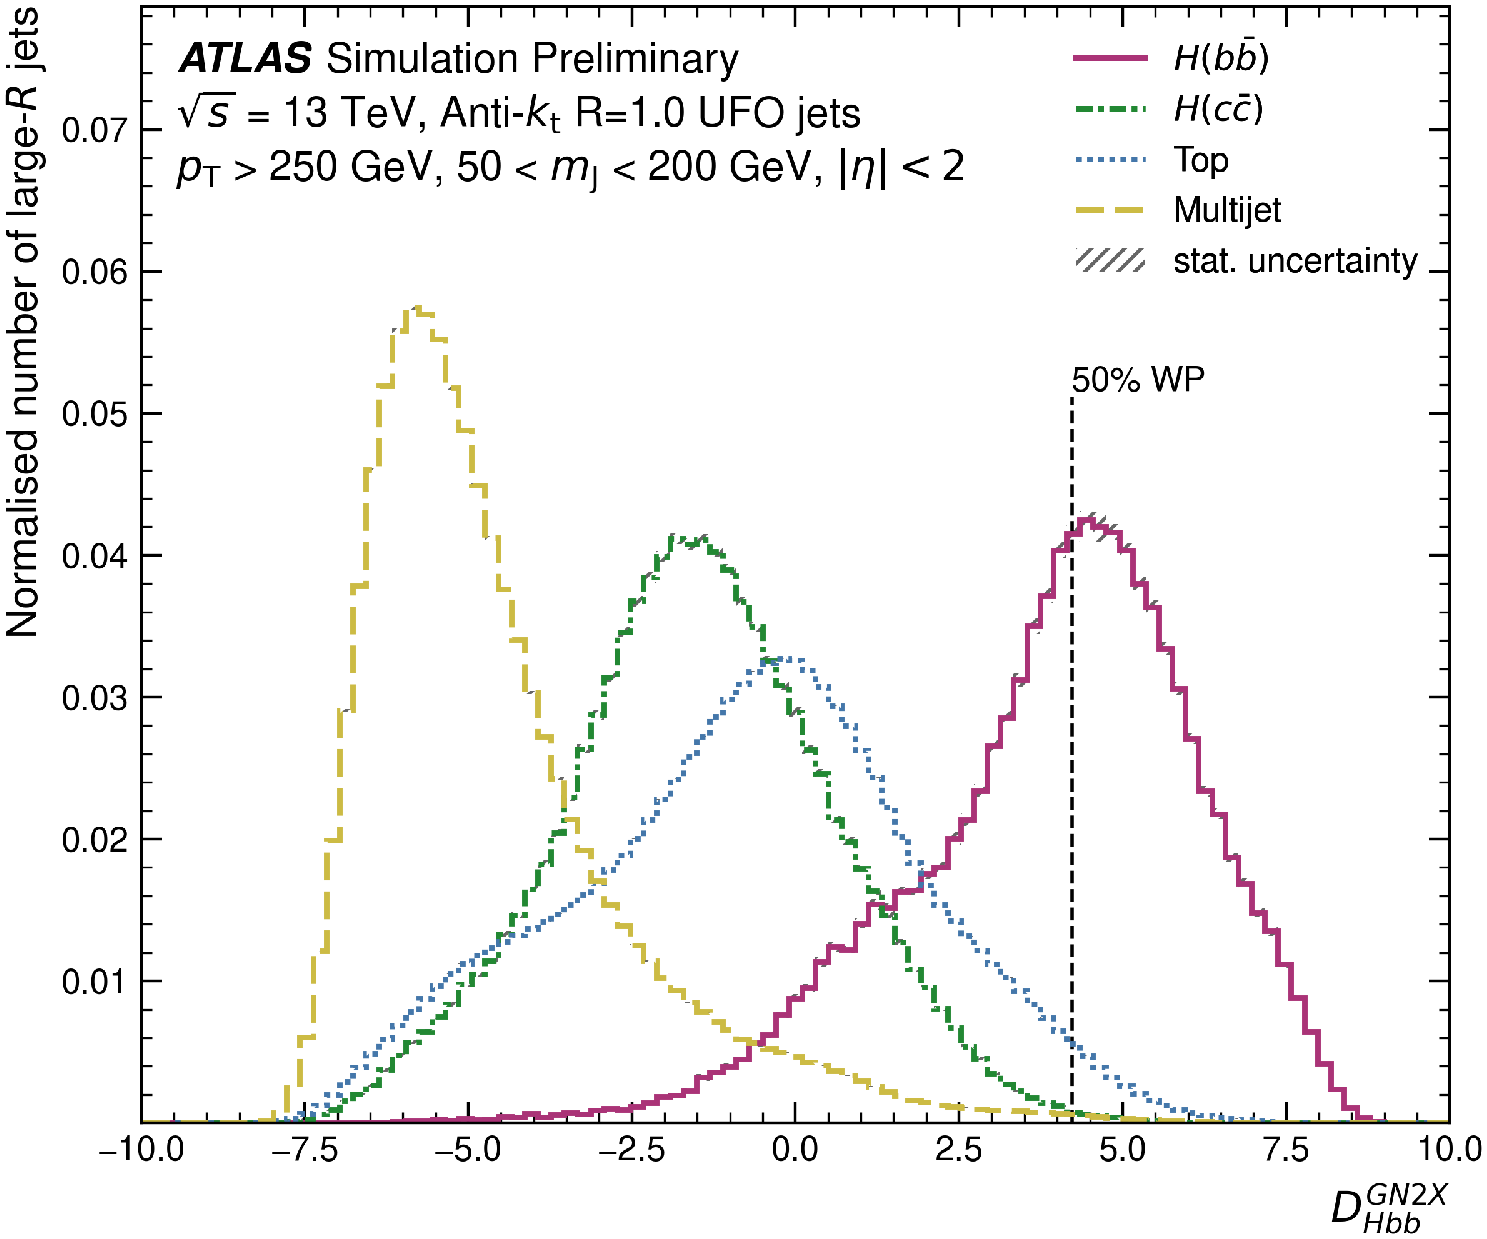
\includegraphics[width=0.5\linewidth]{figures/chapter4/DXbb.png}
	\caption{Normalized $D^{\text{GN2X}}_{Hbb}$ discriminant distributions for $H(b\bar{b})$,
		$H(c\bar{c})$, top, and multijet jet classes, evaluated on SM samples with $p_{\text{T}} > 250$
		GeV and $50 < m_{J} < 200$ GeV. The dashed vertical line indicates the cut corresponding to
		the 50\% $H(b\bar{b})$ signal efficiency working point.}
	\label{fig:GN2X_Discriminant}
\end{figure}

https://atlas.web.cern.ch/Atlas/GROUPS/PHYSICS/PUBNOTES/ATL-PHYS-PUB-2023-021/

https://cds.cern.ch/record/2774902/files/ATL-COM-PHYS-2021-435.pdf

https://xbb-docs.docs.cern.ch

https://ftag.docs.cern.ch

\subsection{Benchmarks and Results -- Boosted}

The performance of \texttt{GN2X} is evaluated in terms of background rejection as a function of
signal efficiency for both $H(b\bar{b})$ and $H(c\bar{c})$ tagging, compared against the DXbb
tagger and a double-tagging baseline using two VR subjets tagged independently with \texttt{GN2},
as shown in Figure~\ref{fig:GN2X:ROC}.

At a 50\% $H(b\bar{b})$ signal efficiency, \texttt{GN2X} achieves rejection factors of
approximately 40 against top-quark jets and 300 against multijet events, corresponding to
improvements of factors of 1.6 and 2.5 respectively over DXbb~\cite{ATL-PHYS-PUB-2023-021}.
For $H(c\bar{c})$ tagging at 50\% signal efficiency, \texttt{GN2X} improves upon the VR subjet
baseline by factors of 3, 5, and 6 in top, multijet, and $H(b\bar{b})$ rejection
respectively~\cite{ATL-PHYS-PUB-2023-021}.

An additional advantage of \texttt{GN2X} is its stable signal efficiency as a function of jet
$p_\text{T}$: \texttt{GN2X} maintains approximately 50\% $H(b\bar{b})$ signal efficiency across
the full $p_\text{T}$ spectrum, whereas DXbb degrades from 50\% at 250~GeV to approximately 35\%
at 1.5~TeV. This is a direct consequence of operating on tracks rather than fixed-size subjet
discriminants, which become less reliable at high boost.

The performance gains over both baselines stem from \texttt{GN2X} having direct access to all
charged particle tracks within the large-$R$ jet simultaneously. The double-tagging baseline tags
subjets independently and therefore cannot capture inter-subjet correlations, while DXbb operates
on high-level subjet discriminants rather than low-level tracks. By operating directly on tracks,
\texttt{GN2X} exploits the full spatial and kinematic correlations between decay products of both
$b$- and $c$-hadrons within the jet.

\begin{figure}[h]
	\centering
	\begin{subfigure}[c]{.35\textwidth}
		\centering
		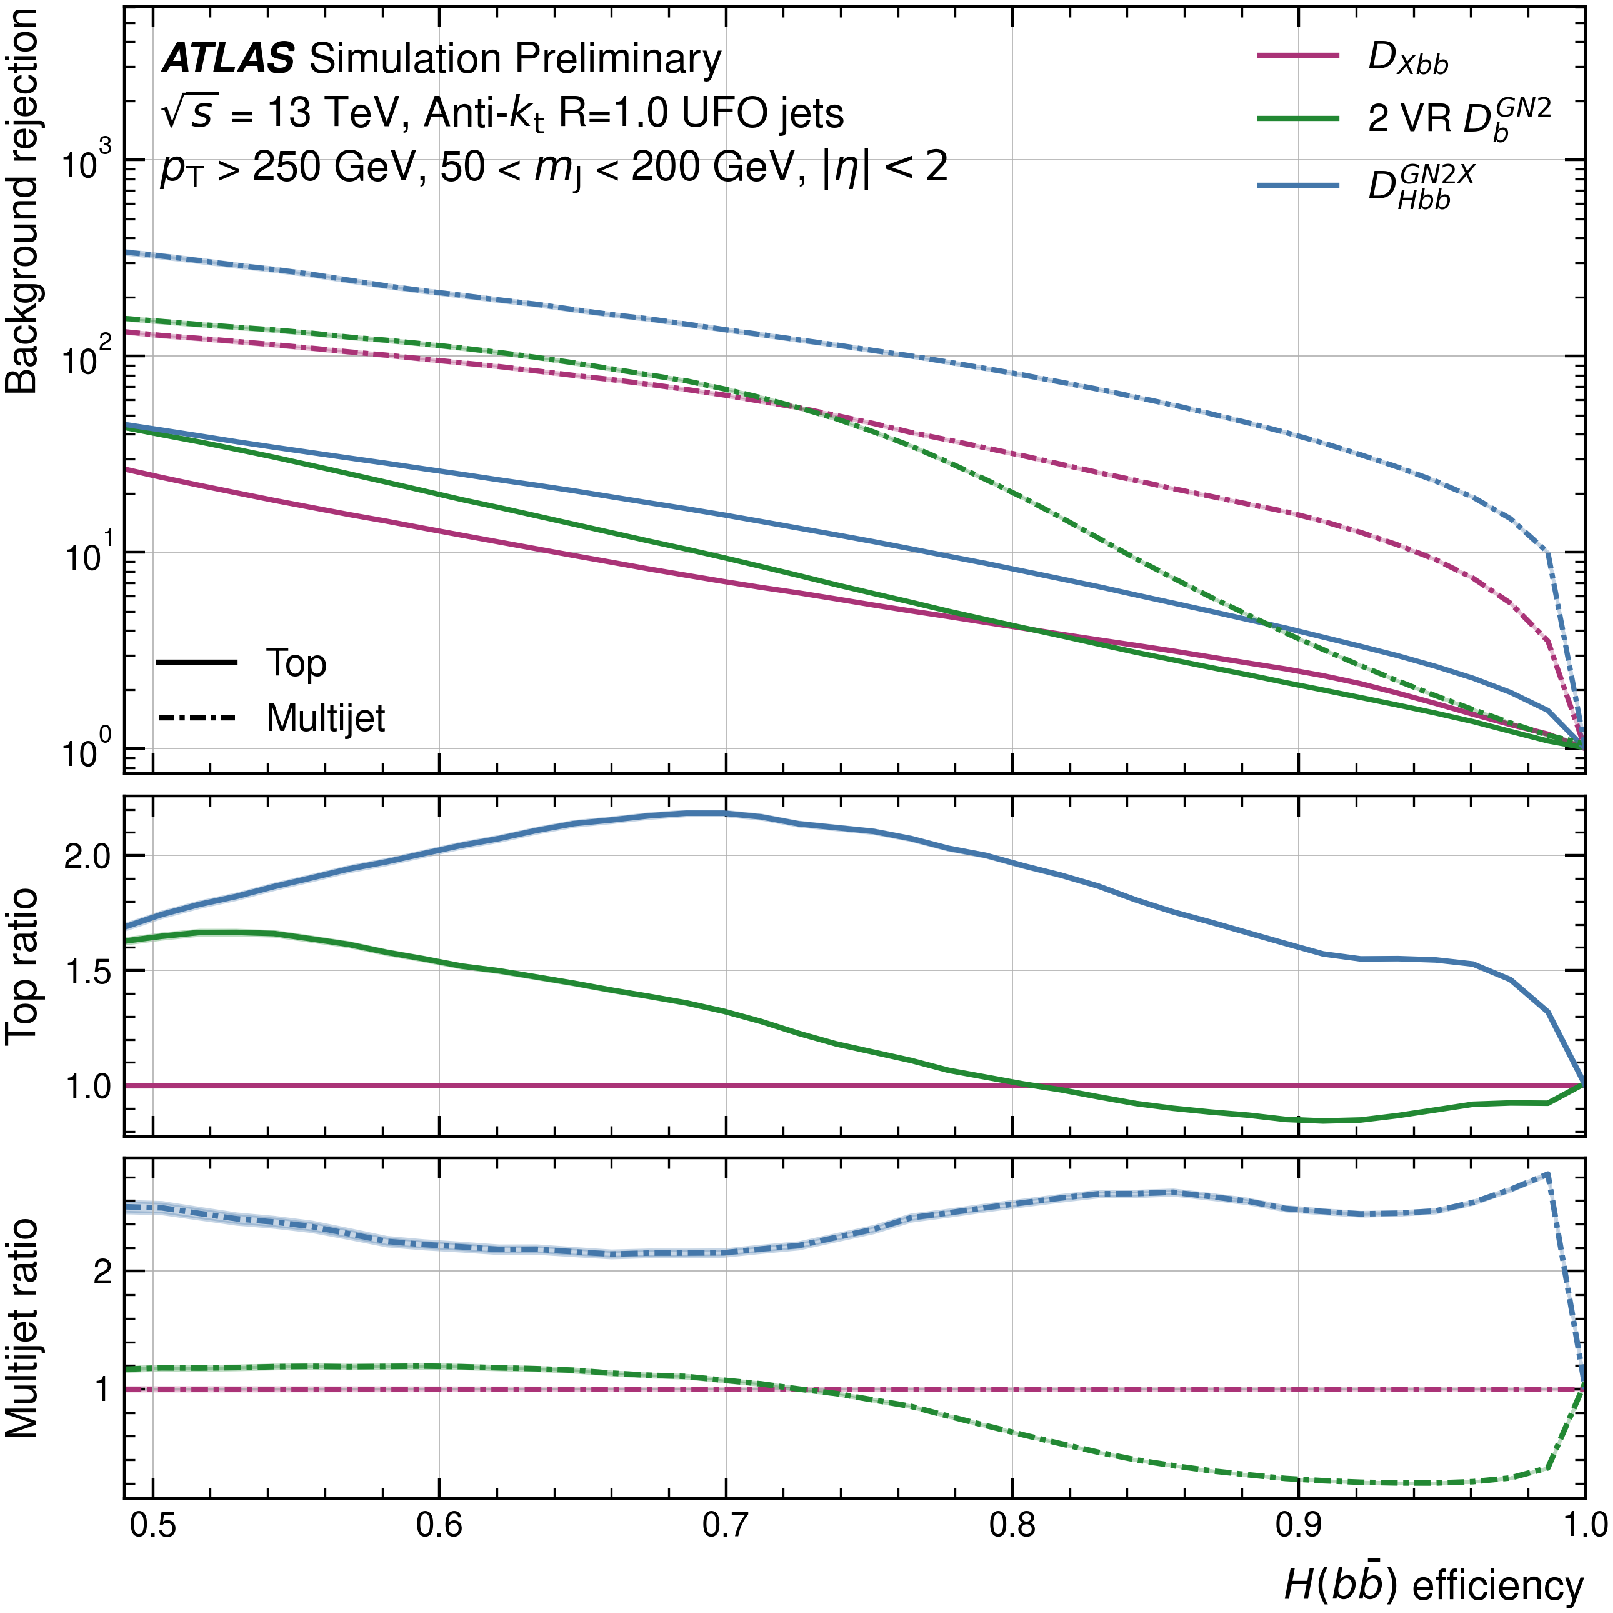
\includegraphics[width=\linewidth]{figures/chapter4/boosted_hbb.png}
		\caption{}
		\label{fig:GN2X:Hbb_ROC}
	\end{subfigure}
	\hspace{0.1\textwidth}   % <-- space here
	\begin{subfigure}[c]{.35\textwidth}
		\centering
		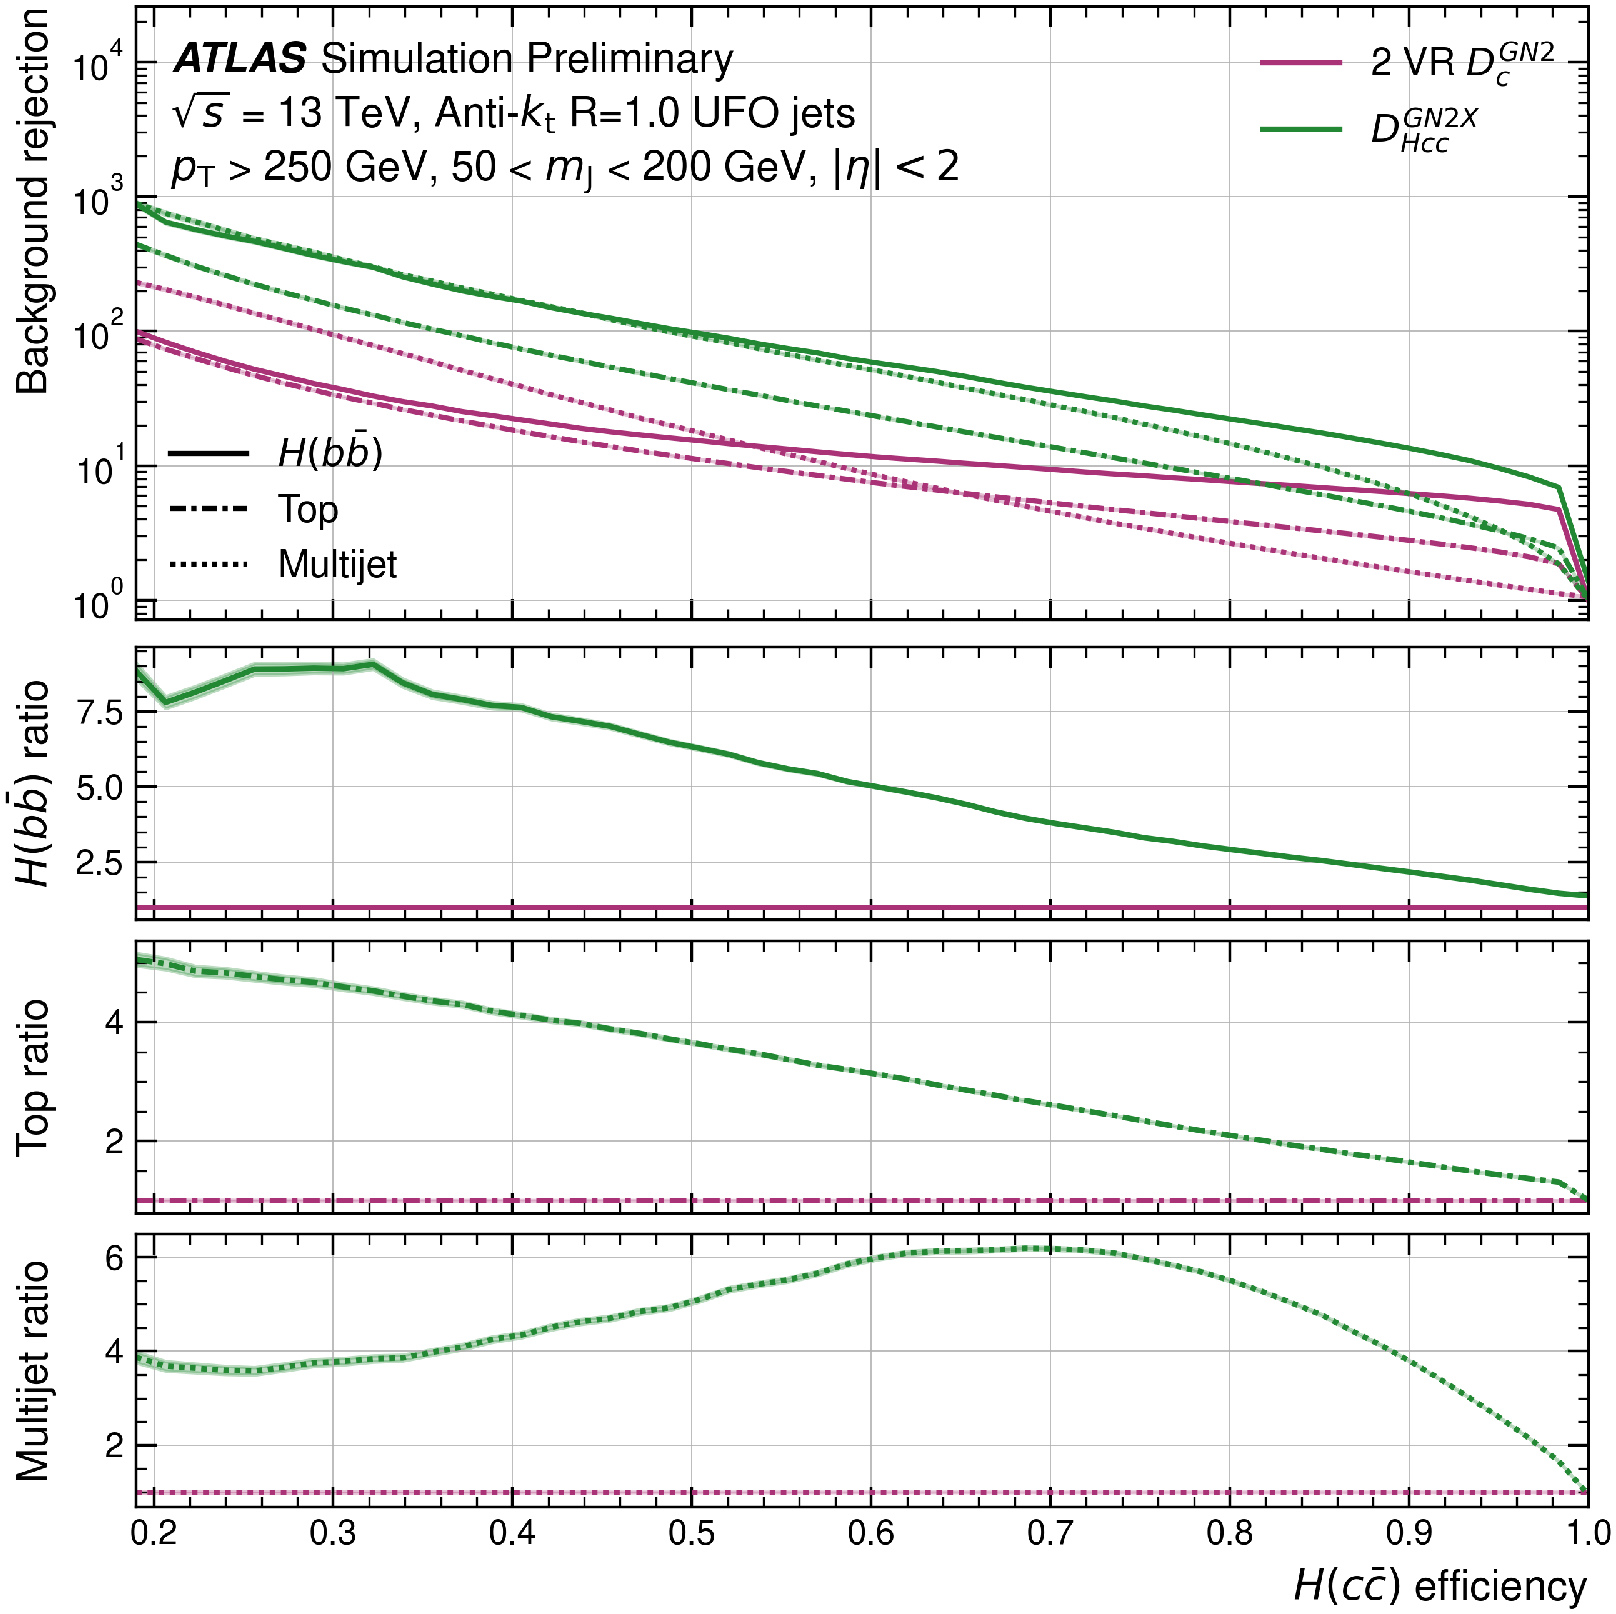
\includegraphics[width=\linewidth]{figures/chapter4/boosted_hcc.png}
		\caption{}
		\label{fig:GN2X:Hcc_ROC}
	\end{subfigure}
	\caption{https://atlas.web.cern.ch/Atlas/GROUPS/PHYSICS/PLOTS/FTAG-2023-01/}
	\label{fig:GN2X:ROC}
\end{figure}

\subsubsection{Mass Sculpting of Background}

An important consideration when deploying any tagger is the potential for mass sculpting, 
where correlations between the tagger score and the large-$R$ jet mass cause the background 
mass distribution to resemble that of the signal after applying a discriminant cut. This is 
particularly undesirable for data-driven background estimation techniques which rely on 
smoothly-falling mass distributions.

Figure~\ref{fig:mass_sculpting} shows the large-$R$ jet mass distributions for $H(b\bar{b})$ 
and multijet samples before and after applying a 70\% $H(b\bar{b})$ efficiency 
$D^{\text{GN2X}}_{Hbb}$ cut. Close to the peak of the $H(b\bar{b})$ mass distribution, 
the multijet mass shape remains largely unchanged, as desired. Some sculpting is observed 
at high and low mass values, attributed to low training statistics in those 
regions~\cite{ATL-PHYS-PUB-2023-021}.

\begin{figure}[htbp]
	\centering
	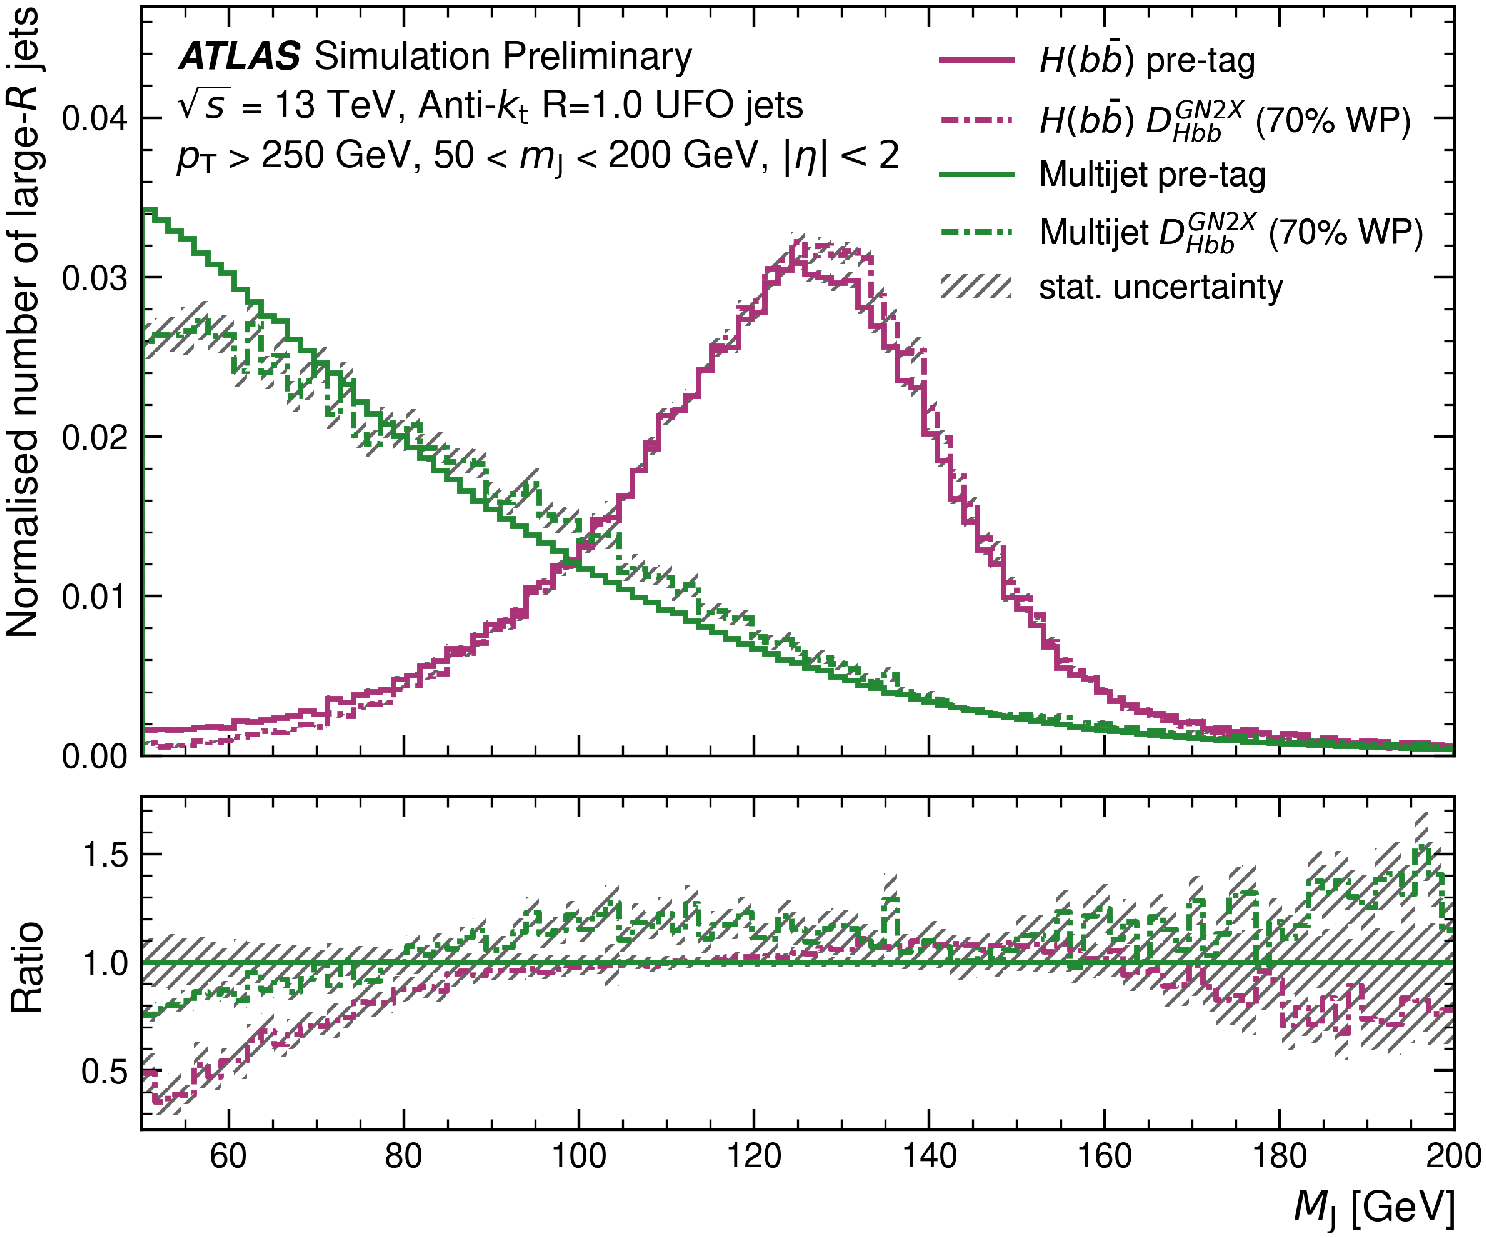
\includegraphics[width=0.5\linewidth]{figures/chapter4/mass_sculpting.png}
	\caption{Large-$R$ jet mass distributions for $H(b\bar{b})$ and multijet samples, before 
		and after applying a 70\% $H(b\bar{b})$ efficiency $D^{\text{GN2X}}_{Hbb}$ cut. Taken 
		from~\cite{ATL-PHYS-PUB-2023-021}.}
	\label{fig:mass_sculpting}
\end{figure}

\section{Calibration of B-Tagging Algorithms}

Since these taggers are trained on Monte Carlo (MC) simulation where truth labels are available, 
and MC is not a perfect model of data, mismodeling effects can arise from multiple sources 
including the matrix element generator, parton shower, detector simulation, and reconstruction. 
As a result, a working point defined in MC does not perfectly extrapolate to the same signal and 
background efficiencies in data. To quantify and correct for these differences, a calibration 
procedure must be performed to account for any excess or deficit of events in data relative to MC.

The GN2X tagger is trained on Monte Carlo simulated events, and therefore its efficiency
may differ between simulation and data due to mismodeling effects. To account for this,
data-to-simulation efficiency scale factors (SFs) are derived, defined as the ratio of the
tagging efficiency measured in data to that predicted by simulation:

\begin{equation}
	SF = \frac{\epsilon^{\text{data}}}{\epsilon^{\text{MC}}}
\end{equation}

These scale factors are measured separately for signal-like and background-like topologies,
since the tagger response depends on the flavor composition and kinematics of the jet.
Two calibrations are described in this section: a signal efficiency calibration using
$Z \rightarrow b\bar{b}$ events, and a mistag rate calibration using semi-leptonic
$t\bar{t}$ events.

\subsection{\texorpdfstring{$Z \rightarrow b\bar{b}$}{Z->bb} Signal Efficiency Calibration}

The signal efficiency calibration targets the tagger's ability to correctly identify
large-$R$ jets originating from a massive particle decaying to a $b\bar{b}$ pair. Since
the Higgs boson is itself the signal of interest in many analyses, it cannot be used
directly for calibration. Instead, $Z \rightarrow b\bar{b}$ events serve as a proxy:
the $Z$ boson is a color-singlet resonance with a mass close to the Higgs boson mass,
and therefore the kinematic properties of $Z \rightarrow b\bar{b}$ and
$H \rightarrow b\bar{b}$ jets are expected to be similar, making the derived scale
factors transferable.

The scale factor is expressed as the ratio of two signal strengths, measured before
and after the tagger requirement is applied:

\begin{equation}
	SF = \frac{\mu_{\text{post-tag}}}{\mu_{\text{pre-tag}}}
\end{equation}

where $\mu$ denotes the number of signal events observed in data divided by the number
predicted by simulation. The pre-tag signal strength $\mu_{\text{pre-tag}}$ is measured
using the clean leptonic decay channel $Z \rightarrow \ell^+\ell^-$, which has
substantially smaller relative backgrounds than the hadronic channel and allows the
$Z \rightarrow b\bar{b}$ yield before tagging to be estimated indirectly. The post-tag
signal strength $\mu_{\text{post-tag}}$ is extracted from a likelihood fit to the
large-$R$ jet mass distribution after applying the tagger requirement, using the
$Z \rightarrow b\bar{b}$ mass peak as a discriminating feature.

Two complementary event selections are used depending on the transverse momentum of
the $Z$-boson candidate. At lower transverse momenta ($200 < p_T < 450$ GeV),
$Z(\rightarrow b\bar{b})\gamma$ events are used, where an associated photon provides
a clean trigger and recoil signature. At higher transverse momenta ($p_T > 450$ GeV),
$Z(\rightarrow b\bar{b}) + \text{jets}$ events are used, where the large-$R$ jet is
sufficiently boosted to be captured within the $R = 1.0$ jet cone.

\subsection{\texorpdfstring{$t\bar{t}$}{ttbar} Mistag Calibration}

Top quark decay is a major source of background for GN2X $H \rightarrow b\bar{b}$ and
$H \rightarrow c\bar{c}$, and therefore it is an important background to calibrate.
As part of my ATLAS authorship qualification task, I investigated the $t\bar{t}$ mistag
rate, which quantifies the rate at which $t\bar{t}$ events pass the predefined working
point selections. The mistag rate is not the same in MC and data due to mismodeling
effects, and so scale factors are derived as defined above.

Efficiency here is defined as the number of $t\bar{t}$ events passing the tagger
selection divided by the total number of $t\bar{t}$ events. Since the number of
$t\bar{t}$ events in data is unknown, it must be extracted by performing a maximum
likelihood fit. In each region (defined later) we perform a counting experiment based
on the requirement that the number of expected MC events should match the number of
events observed in data. Since MC does not perfectly agree with data, we have two
degrees of freedom: $\mu$ and $SF$. Here $\mu$ is the $t\bar{t}$ normalization factor
that accounts for the overall normalization difference between MC and data, and $SF$
is the factor that accounts for the discrepancy introduced by the tagger. With these
two unknowns, we construct two equations (one for the signal region and one for the
control region) to simultaneously extract $\mu$ and $SF$:

\begin{align}
	N^{\text{data}}_{\text{tag}}   &= \mu \cdot \frac{\epsilon^{\text{data}}}{\epsilon^{\text{MC}}} \cdot N^{t\bar{t}}_{\text{tag}} + N^{\text{other}}_{\text{tag}} \\
	N^{\text{data}}_{\text{untag}} &= \mu \cdot \frac{1 - \epsilon^{\text{data}}}{1 - \epsilon^{\text{MC}}} \cdot N^{t\bar{t}}_{\text{untag}} + N^{\text{other}}_{\text{untag}}
\end{align}

Or equivalently, written in terms of scale factors:

\begin{align}
	N^{\text{data}}_{\text{tag}}   &= \mu \cdot SF \cdot N^{t\bar{t}}_{\text{tag}} + N^{\text{other}}_{\text{tag}} \\
	N^{\text{data}}_{\text{untag}} &= \mu \cdot \frac{1 - \epsilon^{\text{MC}} \cdot SF}{1 - \epsilon^{\text{MC}}} \cdot N^{t\bar{t}}_{\text{untag}} + N^{\text{other}}_{\text{untag}}
\end{align}

Since no floating normalization factors are applied to the backgrounds, a region in
phase space must be found where the backgrounds are heavily suppressed and the
$t\bar{t}$ contribution is dominant. To achieve this, semi-leptonic $t\bar{t}$ events
are targeted, where the leptonically decaying top quark serves as the ``tag'' and the
hadronically decaying top quark serves as the ``probe''.

\subsubsection{Tag-and-Probe Event Selection}

Semi-leptonic ttbar decay has a very unique signature in the detector, and reconstructing this topology suppresses many backgrounds. The most dominant background is W+jets followed by single-top, and di-Boson. We use the hadronic largeR jet for the "probe" tagging candidate. The leptonic decaying top is used to as the "tag" candidate. A lepton+MET trigger is used as a foothold into this phase space. By implementing a b-tagging requirement on the "tag" side, we can suppress many of the contributions from W+jets. The feynman diagram shown in \ref{fig:semileptonic_ttbar_diagram}.

\begin{figure}[h]
	\centering
	
\includegraphics[width=0.2\linewidth]{figures/chapter4/ttbar_diagram.png}
	\caption{}
	\label{fig:semileptonic_ttbar_diagram}
\end{figure}

Physics objects are reconstructed and calibrated before event selection. Electrons are required 
to have $p_\text{T} > 28$ GeV, $|\eta_\text{cluster}| < 2.47$ (excluding the barrel/endcap 
transition region $1.37 < |\eta_\text{cluster}| < 1.52$), pass tight identification, and match 
a track in the inner detector (ID). Muons must satisfy $p_\text{T} > 28$ GeV, $|\eta| < 2.5$, 
and pass medium identification by matching ID and muon spectrometer tracks. Both lepton types 
must meet tight isolation criteria and primary vertex compatibility requirements.

Small-$R$ jets are built via the anti-$k_\text{T}$ algorithm ($R = 0.4$) using particle flow 
inputs, requiring $p_\text{T} > 25$ GeV and $|\eta| < 2.5$, with pile-up suppression via the 
Jet Vertex Tagger. $B$-jets are identified using the DL1r multivariate algorithm. Large-$R$ 
jets ($R = 1.0$) are reconstructed from topological LCTopo clusters using the anti-$k_\text{T}$ 
algorithm, then trimmed to reduce pile-up and soft emission effects --- subjets carrying less 
than 5\% of the large-$R$ jet $p_\text{T}$ are removed. Only calibrated jets with 
$p_\text{T} > 300$ GeV and $|\eta| < 2.0$ are considered. Variable-Radius track-jets 
($p_\text{T} > 7$ GeV, $0.02 \leq R \leq 0.4$) are ghost-associated to large-$R$ jets for 
flavor tagging.

\begin{figure}
	\centering
	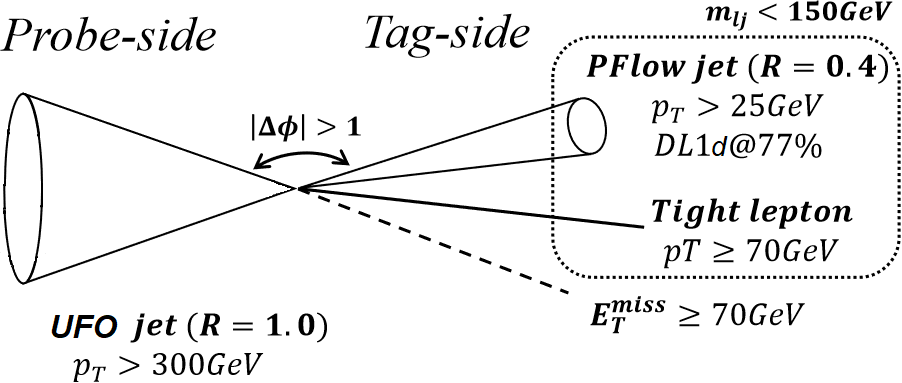
\includegraphics[width=0.6\linewidth]{figures/chapter4/Reco_Event.png}
	\caption{}
	\label{fig:Yields}
\end{figure}

\begin{table}[h]
	\centering
	\resizebox{0.6\textwidth}{!}{%
		\begin{tabular}{ccc}
			\hline
			\textbf{Cut Applied} & \textbf{Electron Channel} & \textbf{Muon Channel} \\
			\hline
			Initial Events                   & 8,911,000 & 8,911,000 \\
			Primary Vertex                   & 8,910,952 & 8,910,952 \\
			Reconstruction                   & 1,220,162 & 1,220,162 \\
			Lepton $p_T > 25$ GeV            & 374,572   & 400,935   \\
			Tight lepton $> 70$ GeV          & 96,701    & 79,744    \\
			Pflow jet $p_T > 25$ GeV         & 94,826    & 77,999    \\
			UFO large-R jet $p_T > 200$ GeV  & 53,462    & 41,511    \\
			MET                              & 44,089    & 33,959    \\
			\hline
		\end{tabular}%
	}
	\caption{Cutflow table for electron and muon selections.}
	\label{tab:cutflow}
\end{table}

Overlap removal is applied sequentially to prevent double-counting: electrons within 
$\Delta R = 0.01$ of a muon are removed first, followed by jets within $\Delta R = 0.2$ of 
an electron. Electrons within $\Delta R = 0.4$ of a remaining jet are then discarded. Muons 
are rejected if within $\Delta R < 0.04 + 10~\text{GeV}/p_\text{T}(\mu)$ of a jet with three 
or more tracks; otherwise the jet is removed.

The missing transverse momentum ($E_\text{T}^\text{miss}$) is computed as the magnitude of 
the negative vector sum of all calibrated object momenta, plus a track-based soft term matched 
to the primary vertex to ensure resilience against pile-up.

Events must pass a single-electron or single-muon trigger with $p_\text{T} > 28$ GeV, and are 
further required to contain exactly one lepton with $p_\text{T} > 70$ GeV to suppress 
non-prompt lepton backgrounds. $E_\text{T}^\text{miss} > 70$ GeV is imposed to account for 
the neutrino from the leptonic $W$ decay. At least one large-$R$ jet with $p_\text{T} \geq 
300$ GeV must be present, with the leading-$p_\text{T}$ jet designated as the probe-jet 
candidate; its mass is restricted to $50~\text{GeV} \leq m \leq 300~\text{GeV}$ to ensure 
compatibility with the calibrated LCTopo jet mass range. At least one small-$R$ jet, 
specifically the closest to the lepton in $\Delta R$, must pass $b$-tagging at the 77\% DL1r 
working point and serves as the tag-jet, significantly suppressing the $V$+jets background.

%\begin{figure}
%	\centering
%	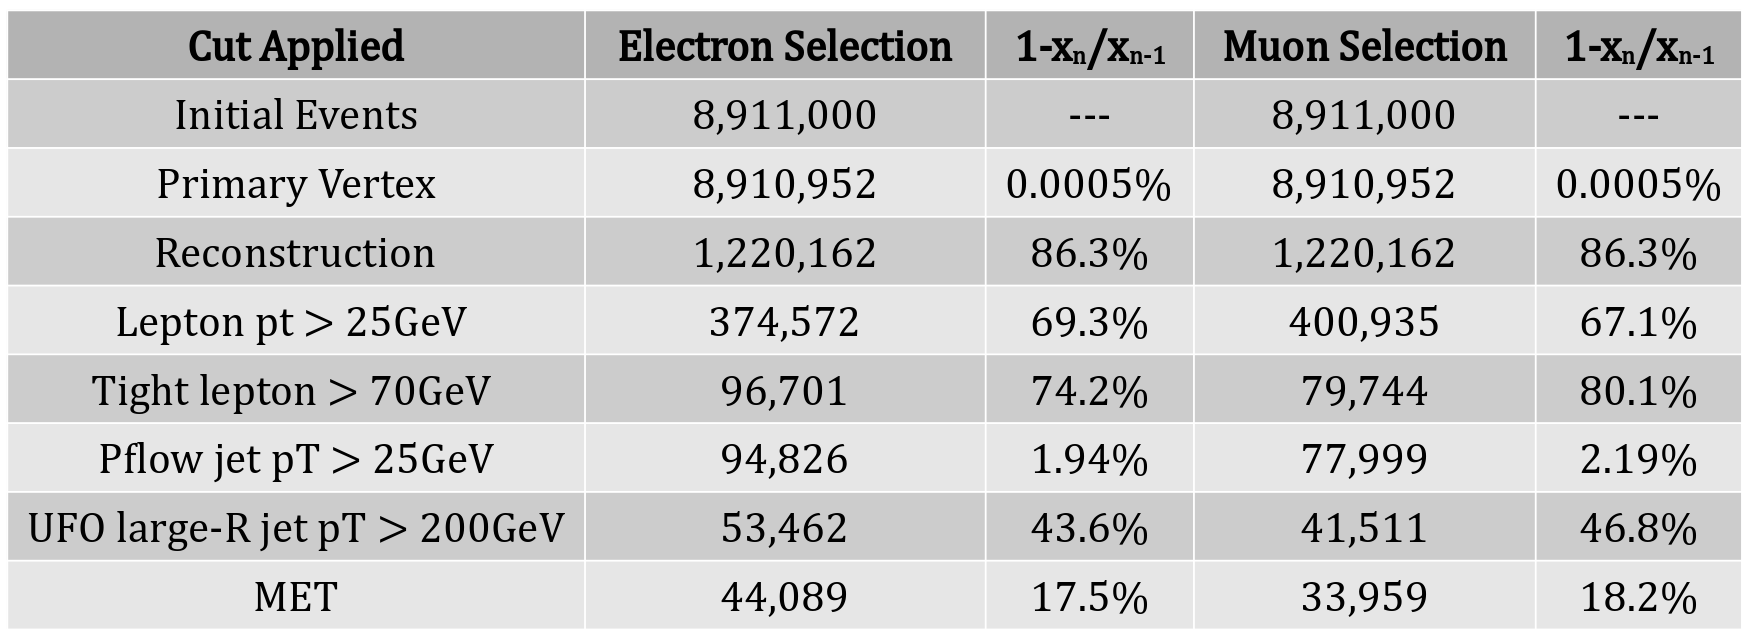
\includegraphics[width=0.7\linewidth]{figures/chapter4/Cutflow.png}
%	\caption{}
%	\label{fig:Yields}
%\end{figure}

%Part of my ATLAS qualification task was ensuring that the largeR jet kinematics matched the previous software release. Switching from LCTopo to UFO is a large change in jet reconstruction. While the $p_T$, $\eta$, and $\phi$ are consistent between the R21 adn R24 software releases, there is a noticeable mass shift in the new release as shown in Figure \ref{fig:probe_jet_validation:subfigd}. To invesigate this mass shift further, validation plots were made in $p_T$ slices as shown in Figure \ref{fig:probe_jet_validation:subfige}, \ref{fig:probe_jet_validation:subfigf}, \ref{fig:probe_jet_validation:subfigg}, \ref{fig:probe_jet_validation:subfigh}. As of the end of my qualification task in 2023, JETMET was still providing updated calibrations to UFO objects to correctly model the mass of top quark.

%\begin{figure}
%	\centering
%	\begin{subfigure}{.24\textwidth}
%		\centering
%		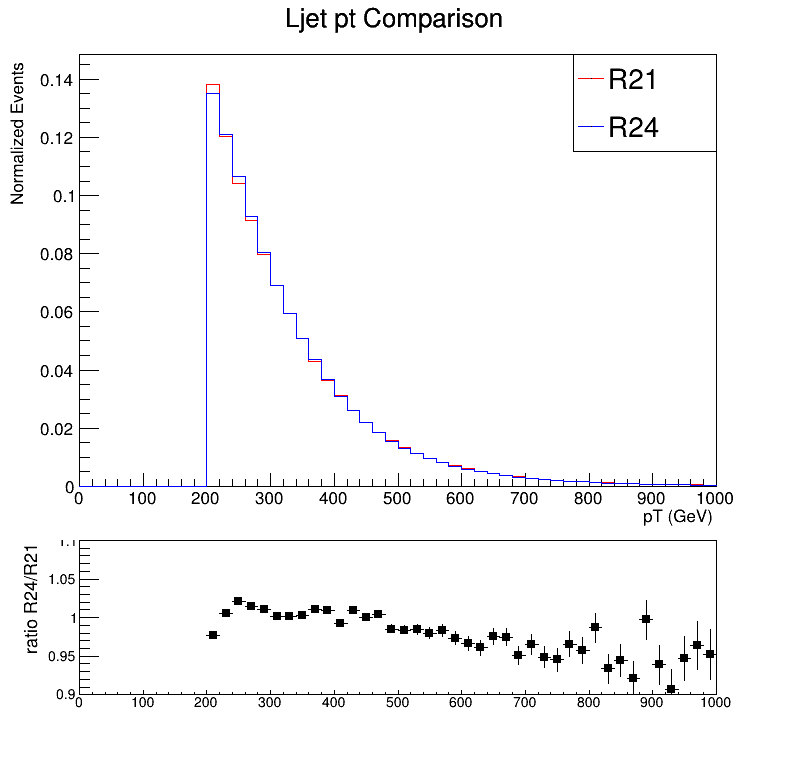
\includegraphics[width=\linewidth]{figures/chapter4/probe_jet_pt.png}
%		\caption{}
%		\label{fig:probe_jet_validation:subfiga}
%	\end{subfigure}%
%	\begin{subfigure}{.24\textwidth}
%		\centering
%		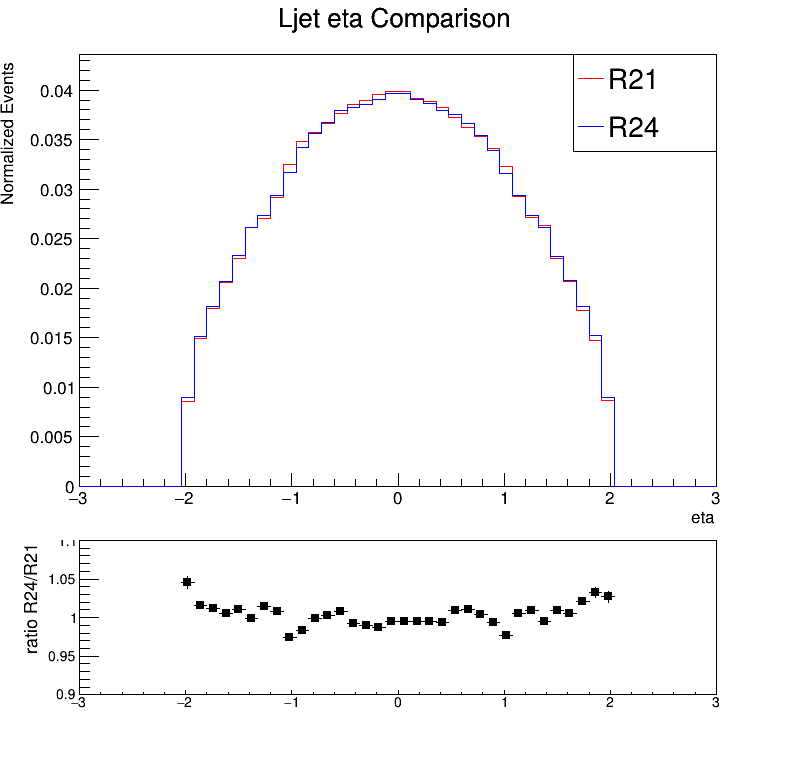
\includegraphics[width=\linewidth]{figures/chapter4/probe_jet_eta.png}
%		\caption{}
%		\label{fig:probe_jet_validation:subfigb}
%	\end{subfigure}
%	\begin{subfigure}{.24\textwidth}
%		\centering
%		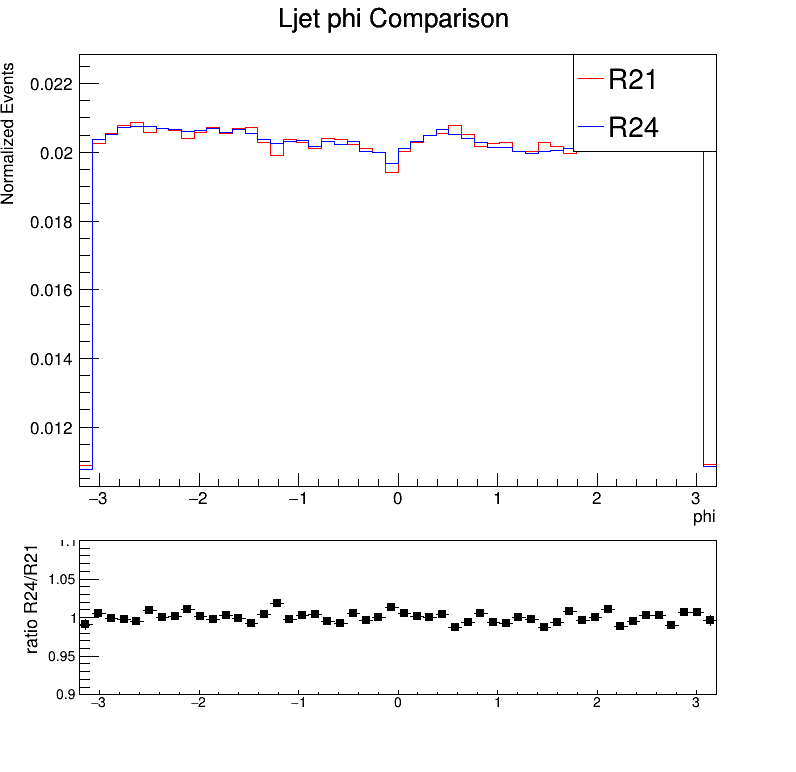
\includegraphics[width=\linewidth]{figures/chapter4/probe_jet_phi.png}
%		\caption{}
%		\label{fig:probe_jet_validation:subfigc}
%	\end{subfigure}
%	\begin{subfigure}{.24\textwidth}
%		\centering
%		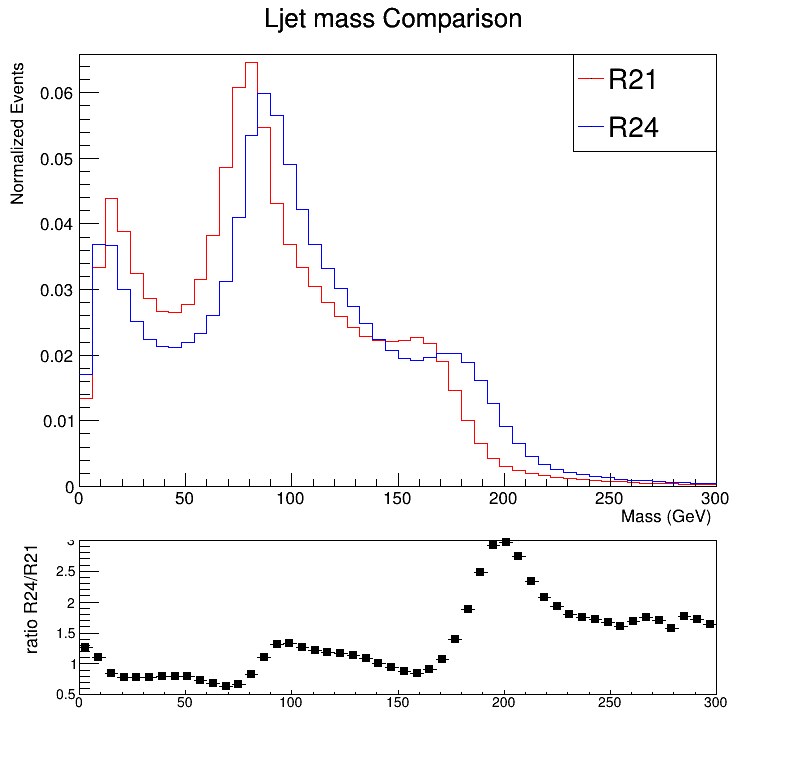
\includegraphics[width=\linewidth]{figures/chapter4/probe_jet_mass.png}
%		\caption{}
%		\label{fig:probe_jet_validation:subfigd}
%	\end{subfigure}
%	\begin{subfigure}{.24\textwidth}
%		\centering
%		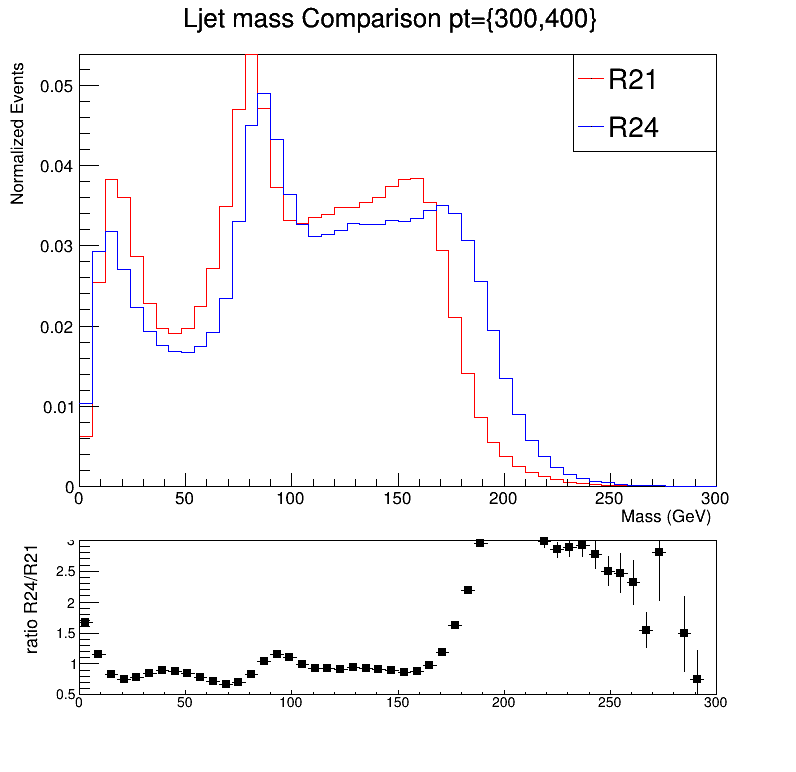
\includegraphics[width=\linewidth]{figures/chapter4/probe_jet_mass_300_400.png}
%		\caption{}
%		\label{fig:probe_jet_validation:subfige}
%	\end{subfigure}%
%	\begin{subfigure}{.24\textwidth}
%		\centering
%		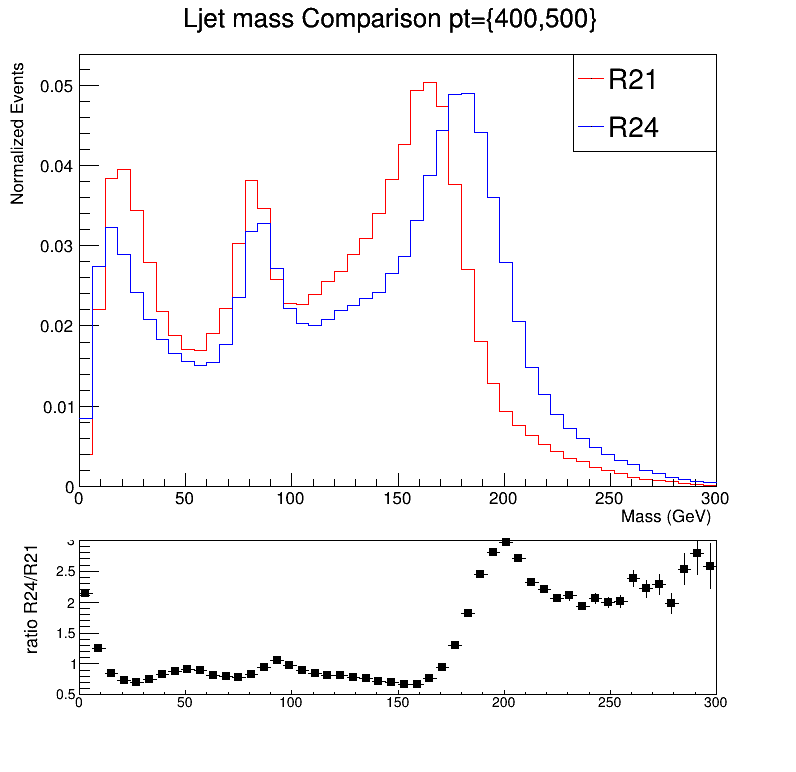
\includegraphics[width=\linewidth]{figures/chapter4/probe_jet_mass_400_500.png}
%		\caption{}
%		\label{fig:probe_jet_validation:subfigf}
%	\end{subfigure}
%	\begin{subfigure}{.24\textwidth}
%		\centering
%		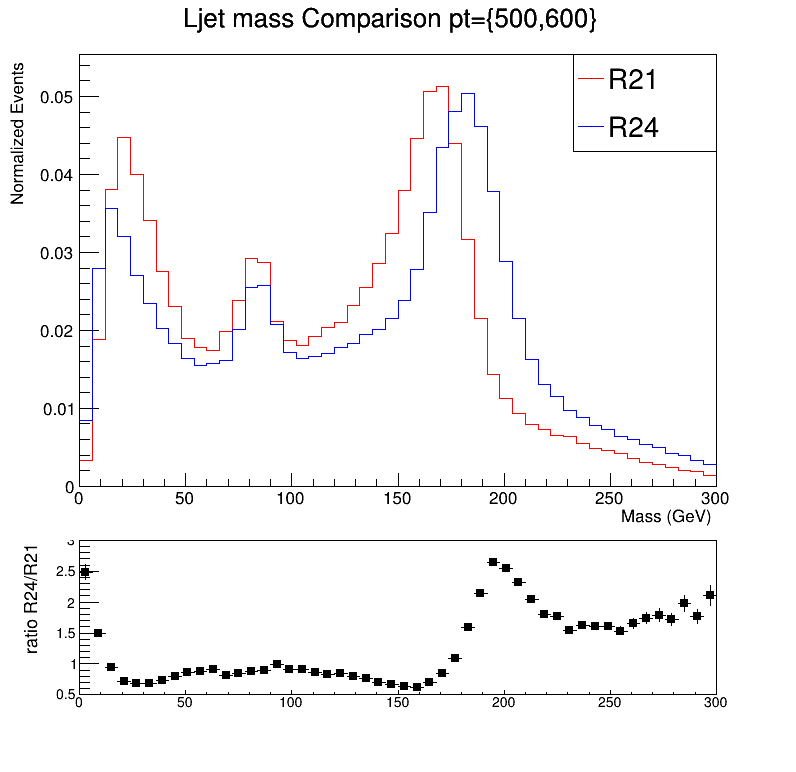
\includegraphics[width=\linewidth]{figures/chapter4/probe_jet_mass_500_600.png}
%		\caption{}
%		\label{fig:probe_jet_validation:subfigg}
%	\end{subfigure}
%	\begin{subfigure}{.24\textwidth}
%		\centering
%		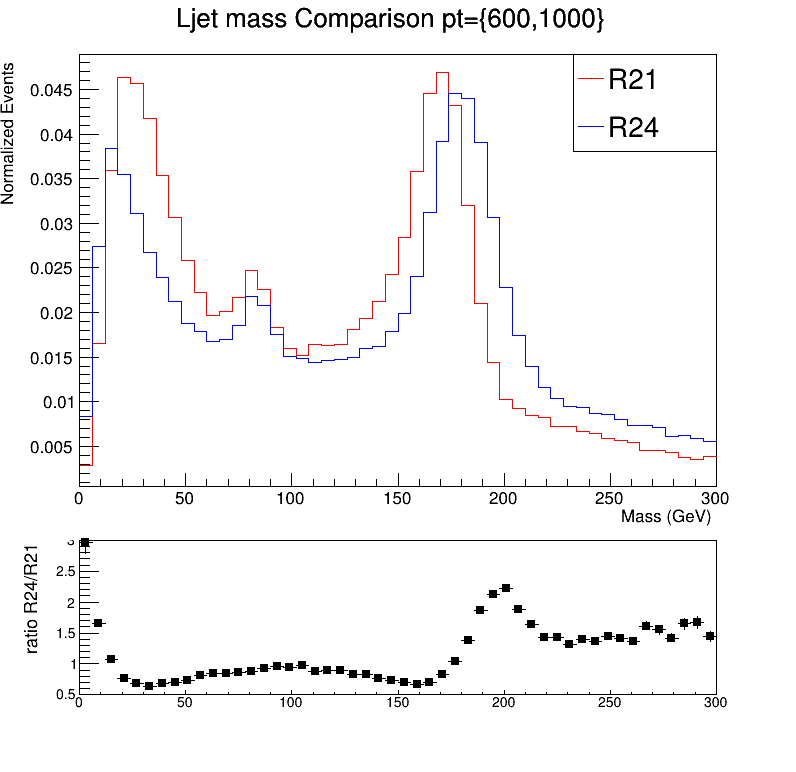
\includegraphics[width=\linewidth]{figures/chapter4/probe_jet_mass_600_1000.png}
%		\caption{}
%		\label{fig:probe_jet_validation:subfigh}
%	\end{subfigure}
%	\caption{}
%	\label{fig:probe_jet_validation}
%\end{figure}

\subsubsection{Constructing Fit Regions}

The goal of this analysis is to measure the mistag efficiency $\epsilon^{data}_{ttbar}$ for different values of $p_T^{probe}$. We can extract the mistag efficiency by fitting the two previously defined parameters: ttbar normalization $\mu$ and SF. The signal regions are defined to have events that pass a given working point for the GN2Xv01 tagger, and control regions are populated with events that fail tagging requirements. As of the time of my qualification task, working points had not yet been finalized so a flat cut at 1.76 was used to approximate the 70\% working point. In recent developments, the GN2X working points are no longer defined as flat cuts on the discriminant. To reduce background sculpting, working points are defined as a function of the discriminant, jet mass, and jet pT.

The post-fit control regions are shown in Figure \ref{fig:ttbar_CR}. Notice that after implementing event selections, the W+jets, single-top, and di-Boson background are heavily suppressed. A consistent theme across control regions show that the low mass bin has about 25\% more data than weighted MC predicts. Since UFO are a newly defined reconstruction technique, I was told to wait for the finalized recommendations. Another observation is the increase in ttbar\_nonmatch as the boost increases. These events, in white, come from QCD jets originating from ISR/FSR during the $2\rightarrow 2$ simulated $q, q \rightarrow t, \bar{t}$ process. 

\begin{figure}[h]
	\centering
	\begin{subfigure}{.32\textwidth}
		\centering
		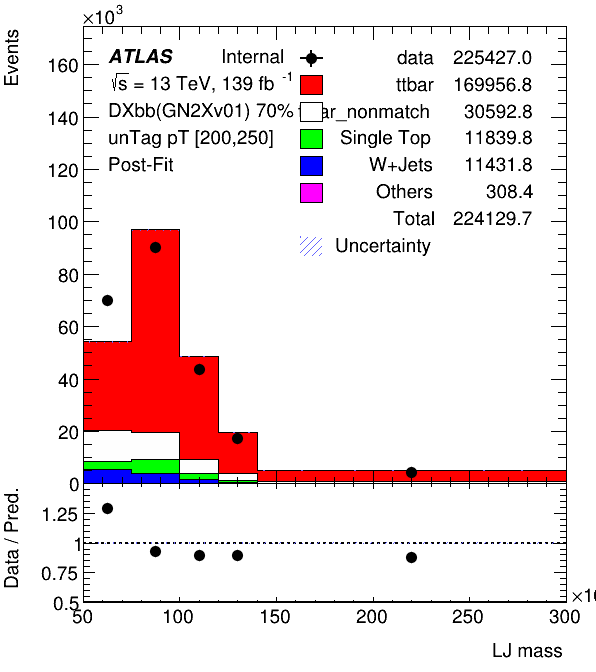
\includegraphics[width=\linewidth]{figures/chapter4/CR_pt_200_postfit.png}
		\caption{}
		\label{fig:sub1}
	\end{subfigure}%
	\begin{subfigure}{.32\textwidth}
		\centering
		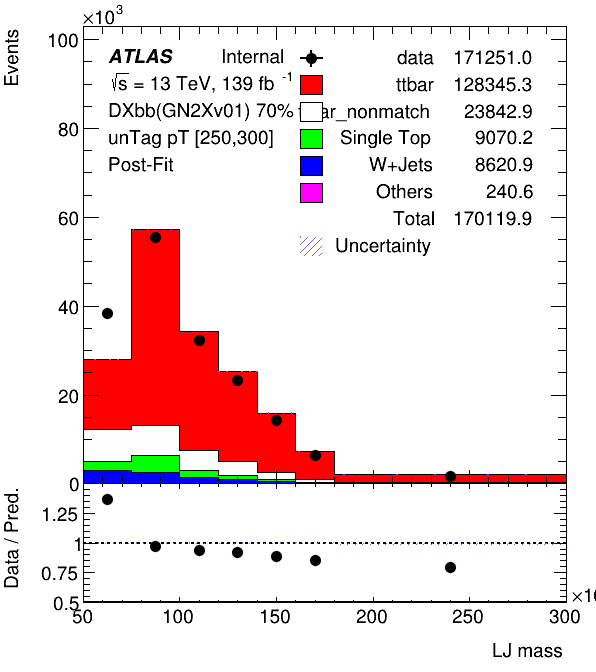
\includegraphics[width=\linewidth]{figures/chapter4/CR_pt_250_postfit.png}
		\caption{}
		\label{fig:sub2}
	\end{subfigure}
	\begin{subfigure}{.32\textwidth}
		\centering
		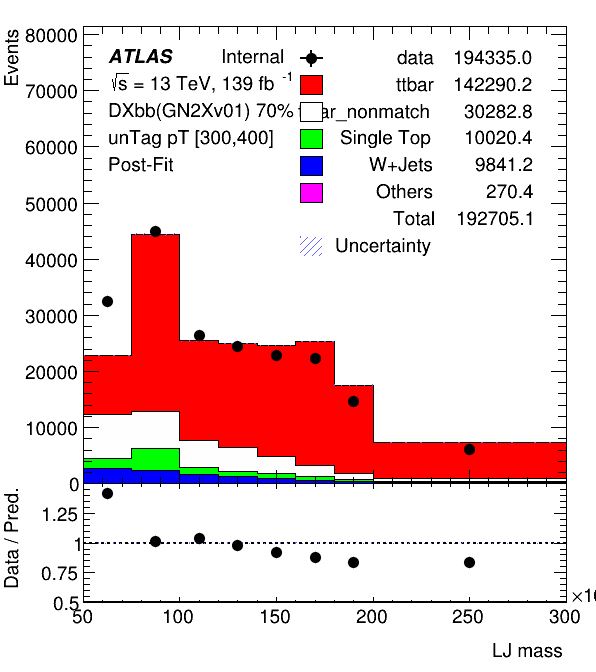
\includegraphics[width=\linewidth]{figures/chapter4/CR_pt_300_postfit.png}
		\caption{}
		\label{fig:sub2}
	\end{subfigure}
	\begin{subfigure}{.32\textwidth}
		\centering
		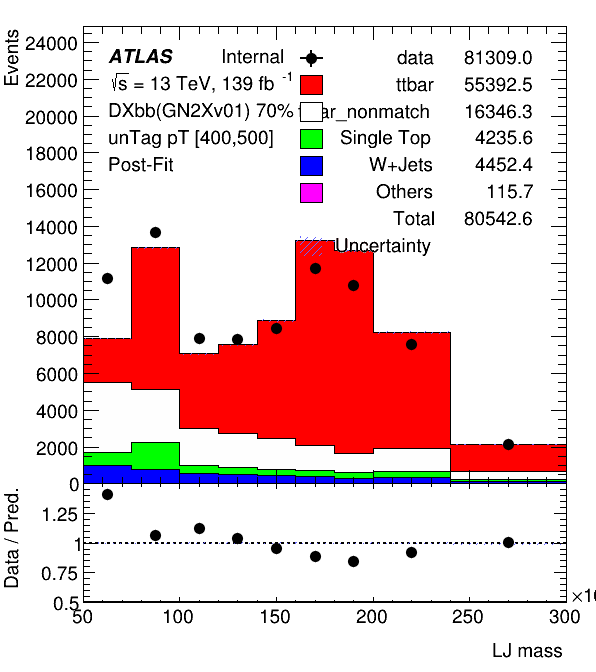
\includegraphics[width=\linewidth]{figures/chapter4/CR_pt_400_postfit.png}
		\caption{}
		\label{fig:sub2}
	\end{subfigure}
	\begin{subfigure}{.32\textwidth}
		\centering
		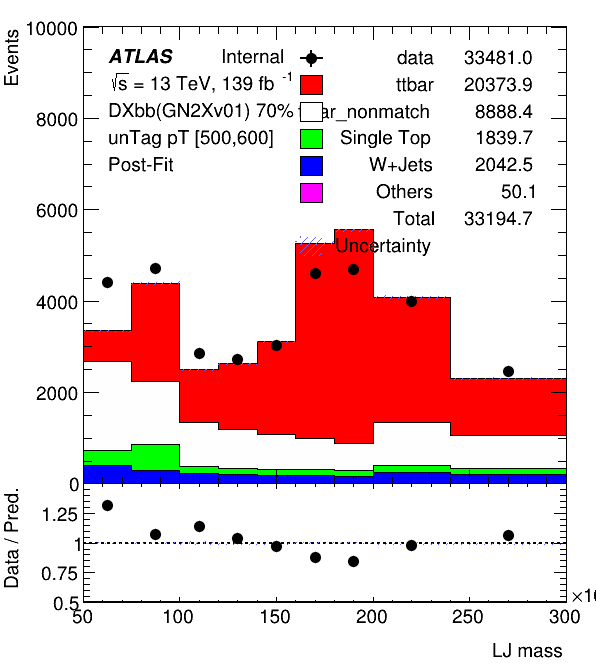
\includegraphics[width=\linewidth]{figures/chapter4/CR_pt_500_postfit.png}
		\caption{}
		\label{fig:sub2}
	\end{subfigure}
	\begin{subfigure}{.32\textwidth}
		\centering
		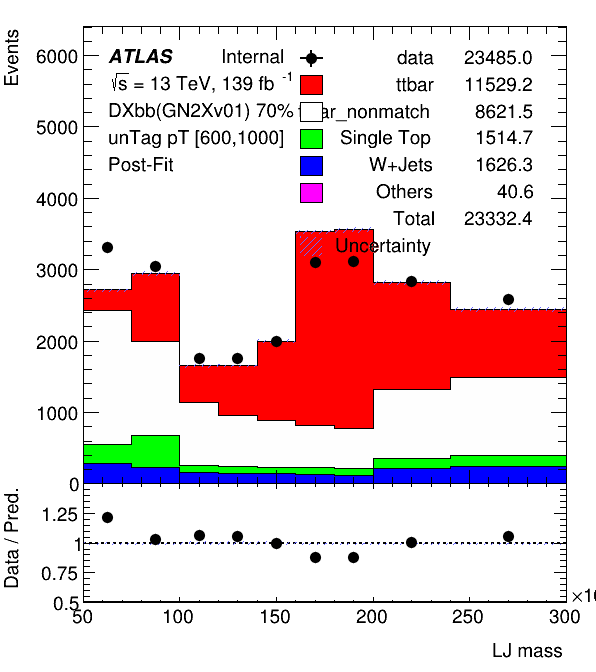
\includegraphics[width=\linewidth]{figures/chapter4/CR_pt_600_postfit.png}
		\caption{}
		\label{fig:sub2}
	\end{subfigure}
	\caption{}
	\label{fig:ttbar_CR}
\end{figure}

The post-fit signal regions are shown in Figure \ref{fig:ttbar_SR}. In general, the data-MC agreement is very good across all bins in all regions. Notice how the ttbar\_nonmatch is not as dominant in the boosted regions as a side-affect of the tagging requirement since QCD is much more suppressed cutting on the disciminant as shown in \ref{fig:GN2X_Discriminant}. Through performing these fits, the ttbar normalization factor $\mu$ and the SF are extracted in each $p_T$ slice. Its important to note that these parameters are extracted simultaneously using the SR and CR in tandom.

\begin{figure}
	\centering
	\begin{subfigure}{.32\textwidth}
		\centering
		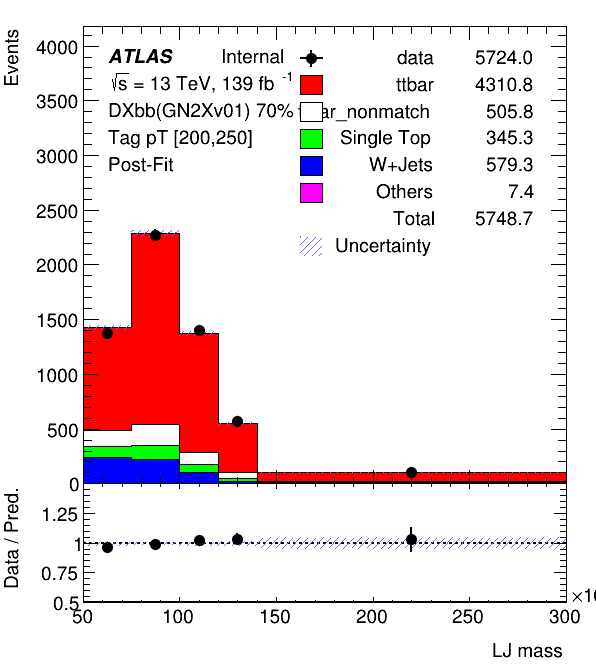
\includegraphics[width=\linewidth]{figures/chapter4/SR_pt_200_postfit.png}
		\caption{}
		\label{fig:sub1}
	\end{subfigure}%
	\begin{subfigure}{.32\textwidth}
		\centering
		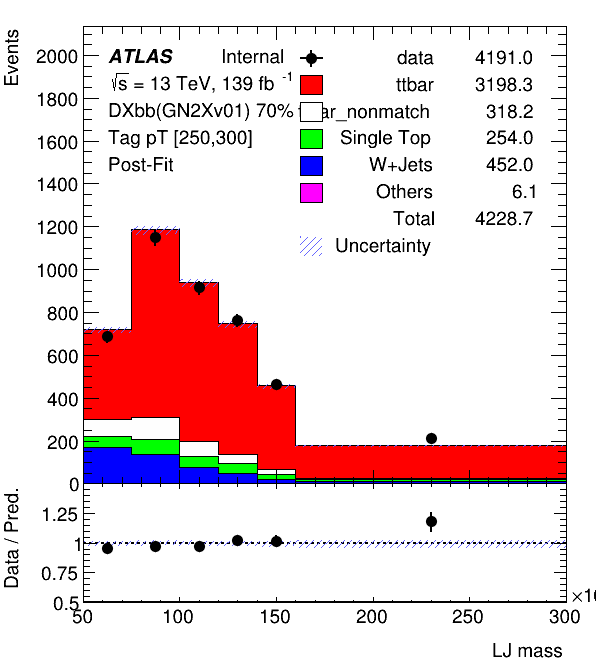
\includegraphics[width=\linewidth]{figures/chapter4/SR_pt_250_postfit.png}
		\caption{}
		\label{fig:sub2}
	\end{subfigure}
	\begin{subfigure}{.32\textwidth}
		\centering
		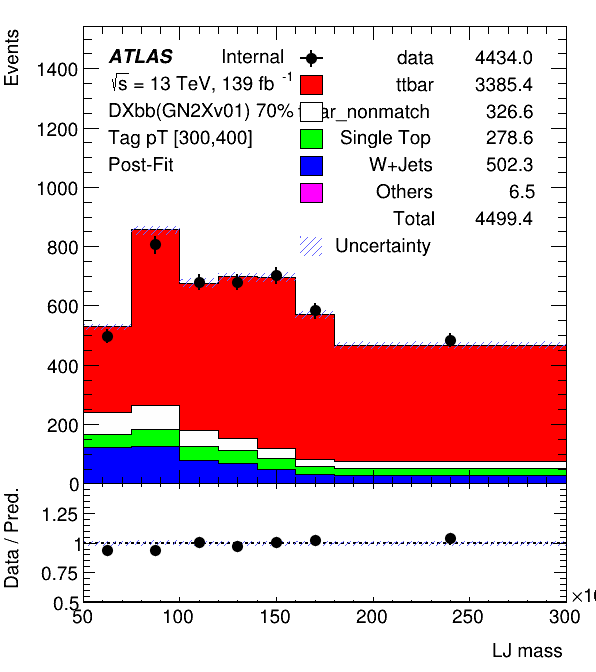
\includegraphics[width=\linewidth]{figures/chapter4/SR_pt_300_postfit.png}
		\caption{}
		\label{fig:sub2}
	\end{subfigure}
	\begin{subfigure}{.32\textwidth}
		\centering
		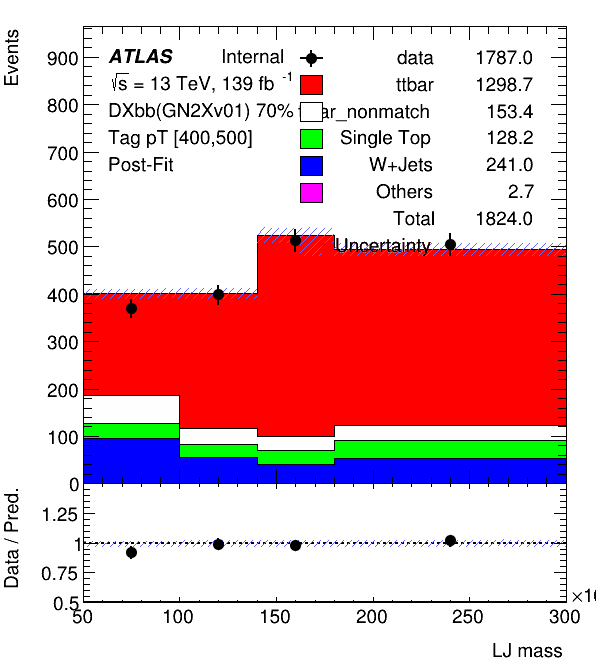
\includegraphics[width=\linewidth]{figures/chapter4/SR_pt_400_postfit.png}
		\caption{}
		\label{fig:sub2}
	\end{subfigure}
	\begin{subfigure}{.32\textwidth}
		\centering
		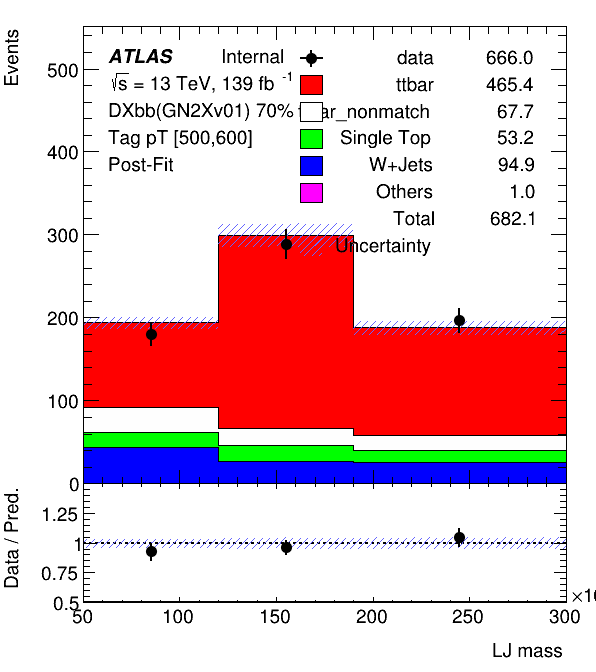
\includegraphics[width=\linewidth]{figures/chapter4/SR_pt_500_postfit.png}
		\caption{}
		\label{fig:sub2}
	\end{subfigure}
	\begin{subfigure}{.32\textwidth}
		\centering
		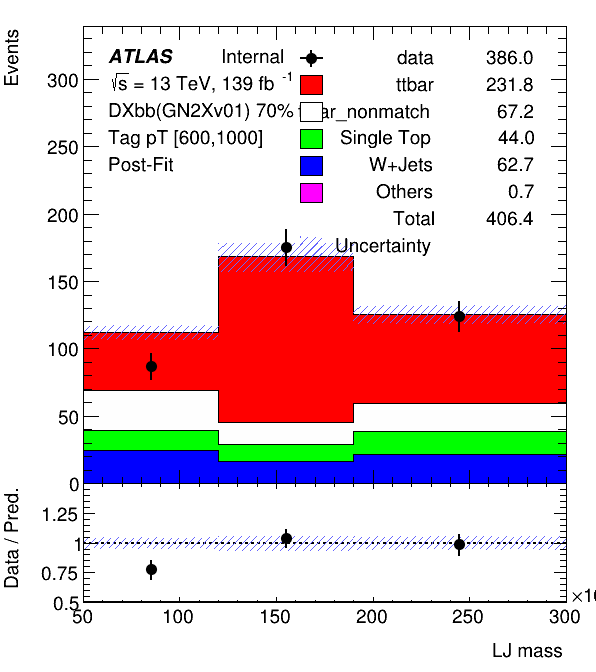
\includegraphics[width=\linewidth]{figures/chapter4/SR_pt_600_postfit.png}
		\caption{}
		\label{fig:sub2}
	\end{subfigure}
	\caption{}
	\label{fig:ttbar_SR}
\end{figure}

\subsubsection{ttbar Mistag Calibration Results}

A normalization factor and SF is derived per $p_T$ region. These parameters are extracted by maximizing the likelihood fit function. This can be interpreted as: what choice of parameters ($\mu$ and SF) yield the highest probability that the observed data matches the predicted MC. These fits only included statistical uncertainties, but a final result would also include systematic uncertainties such as: detector resolution, jet reconstruction, and flavor tagging uncertainties. The stat-only MC-16 results derived on full run 2 dataset are shown in \ref{fig:ttbar_SF:MC16}. The stat-only MC-20 results derived on full run 2 dataset are shown in \ref{fig:ttbar_SF:MC20}. The largest difference between these results are found in the ttbar normalization factors which were significantly lower in MC16 compared to MC20. Despite these differences, the SF between MC16 and MC20 are in much better agreement.

\begin{figure}
	\centering
	\begin{subfigure}{.49\textwidth}
		\centering
		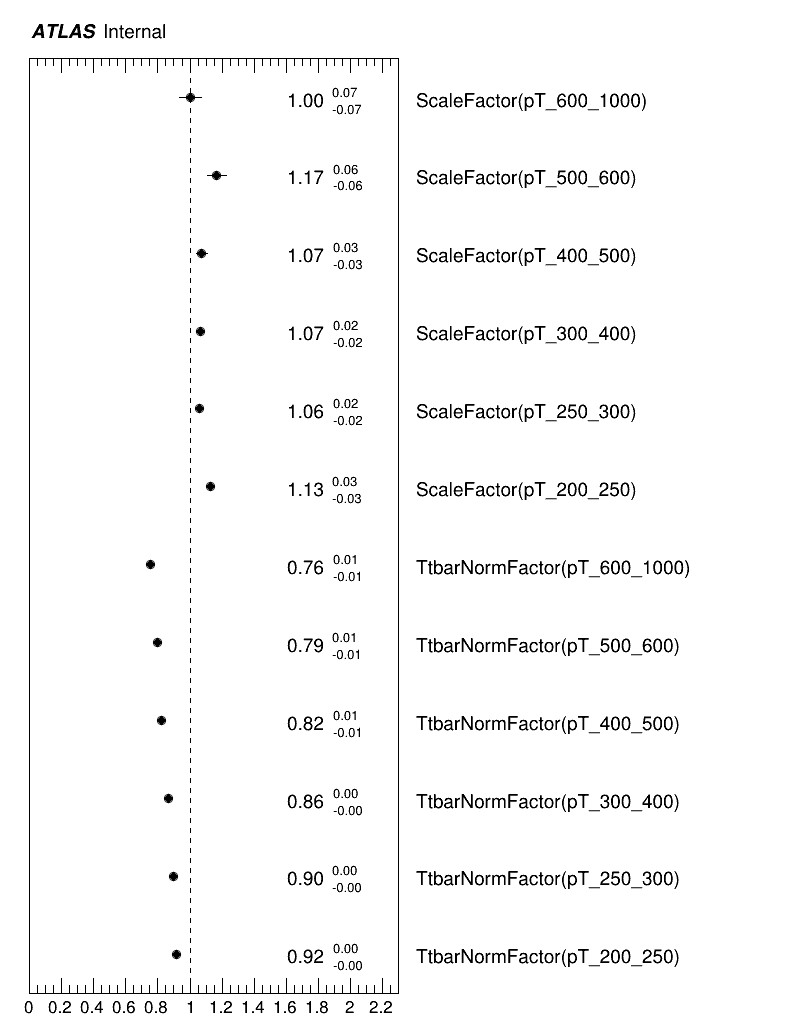
\includegraphics[width=\linewidth]{figures/chapter4/scale_factors_mc16.png}
		\caption{}
		\label{fig:ttbar_SF:MC16}
	\end{subfigure}%
	\begin{subfigure}{.49\textwidth}
		\centering
		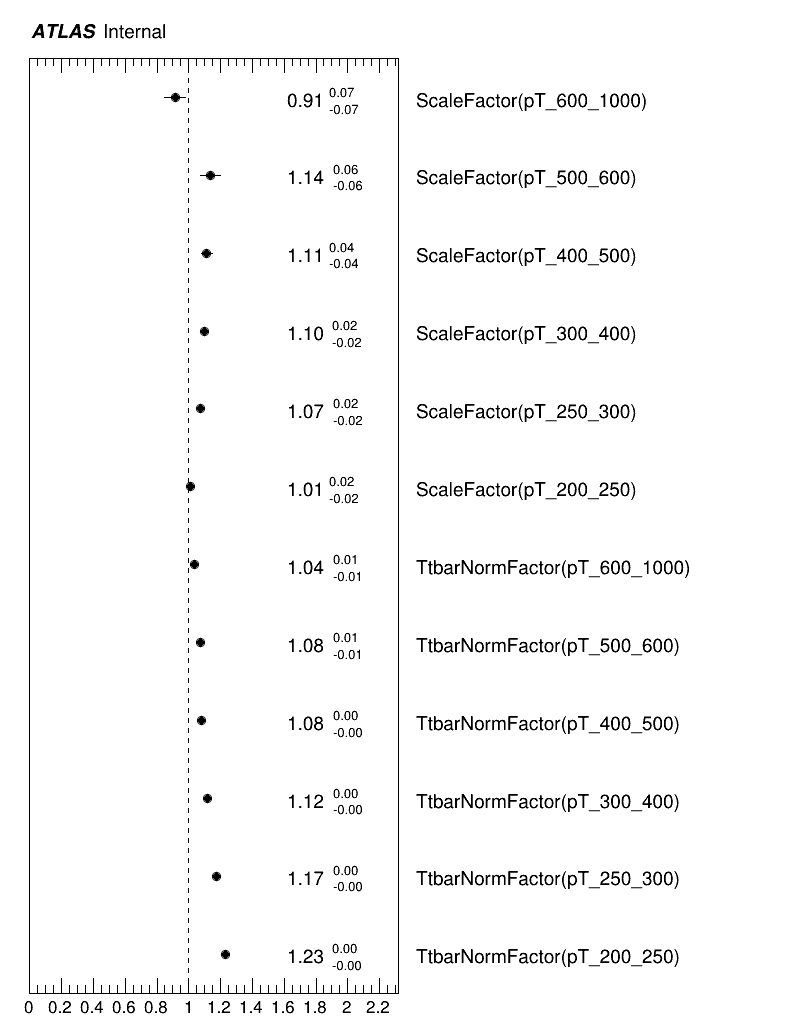
\includegraphics[width=\linewidth]{figures/chapter4/scale_factors_mc20.png}
		\caption{}
		\label{fig:ttbar_SF:MC20}
	\end{subfigure}
	\caption{}
	\label{fig:ttbar_SF}
\end{figure}

\section{Conclusion}

This chapter has traced the evolution of $b$-tagging algorithms in ATLAS from the early
multivariate taggers of Run~2 through to the graph- and attention-based architectures deployed
for Run~3. The progression reflects a consistent trend: each generation of taggers has moved
closer to the raw detector information, replacing hand-engineered summary variables with learned
representations operating directly on tracks, vertices, and hits.

The performance gains from this evolution are summarized in Figure~\ref{fig:history}. These gains have direct physics implications. Higher background rejection at fixed signal
efficiency translates to cleaner $b$-jet samples, reduced systematic uncertainties on flavor
tagging scale factors, and improved sensitivity in analyses that rely on $b$-jet identification
--- from top quark measurements to searches for new phenomena involving heavy-flavor final
states. Looking ahead, further improvements are anticipated through the incorporation of
additional low-level inputs, larger training samples exploiting the full Run~3 dataset, and
continued architectural development motivated by the demands of the High-Luminosity LHC, where
the increased pile-up environment will place even greater demands on the precision and robustness
of flavor tagging algorithms.

This chapter presented the calibration of the GN2Xv01 boosted jet tagger using a 
$t\bar{t}$-enriched region derived from semi-leptonic top quark decays. The tag-and-probe 
event selection strategy proved effective at isolating a high-purity $t\bar{t}$ sample, 
suppressing dominant backgrounds such as $W$+jets and single-top contributions to a 
manageable level. The unique detector signature of semi-leptonic $t\bar{t}$ events, combined 
with a $b$-tagging requirement on the leptonic-side tag jet, provided the clean phase space 
necessary for a reliable extraction of the mistag rate.

The GN2X discriminant was used to construct the signal and control regions, demonstrating 
good data-MC agreement across all probe jet $p_T$ bins after performing the simultaneous 
maximum likelihood fit, successfully extracting the $t\bar{t}$ normalization factor $\mu$ 
and scale factor $SF$ in each $p_T$ slice. Scale factors were derived for both MC16 and MC20 
configurations using the full Run 2 dataset, showing good mutual consistency despite notable 
differences in the extracted normalization factors between the two campaigns. The techniques 
and infrastructure developed here lay the groundwork for a full GN2Xv01 calibration to be 
deployed in future ATLAS Higgs boson analyses targeting boosted $H \rightarrow b\bar{b}$ 
and $H \rightarrow c\bar{c}$ signatures.




